

% ==================
%
% =-------------------
\section{Simulation of the Multidomain Model}\label{sec:solver_multidomain_model}

The multidomain model is an alternative to the fiber based electrophysiology model discussed in the last section.
As introduced in \cref{sec:multidomain_model}, it does not explicitly resolve muscle fibers, but considers activity in the muscle domain in a homogenized view.
On every point in the 3D muscle mesh, separate values $V_m^k$ of the transmembrane potential exist for every MU $k \in \{1,\dots,N_\text{MU}\}$, in addition to the value $\phi_e$ for the extracellular electric potential. 
The computational domain considers the muscle volume $\Omega_M$ and the body domain $\Omega_B$, which represents  adipose tissue on top of the muscle.
To solve the multidomain model, a large linear system has to be solved in every timestep, as described in \cref{sec:discretization_body_domain}.

In the following, \cref{sec:multidomain_components} discusses the model setup for a scenario with four MUs. \Cref{sec:multidomain_simulation_emg} demonstrates a larger simulation scenario with 25 MUs, which can be used to simulate surface EMG signals. We discuss differences between the multidomain approach and the fiber based electrophysiology model in \cref{sec:multidomain_differences}.

\subsection{Components of the Computational Model}\label{sec:multidomain_components}

In the following, we consider a multidomain simulation with muscle and body fat domains and four MUs. We use a muscle mesh with $16 \times 16 \times 74 = \num{18944}$ elements and linear finite element ansatz functions and a fat mesh with $32 \times 4 \times 74 = \num{9472}$ elements, which are partitioned to 128 subdomains for 128 processes. 

The scenario uses the following electric conduction tensors $\bfsigma_i$ and $\bfsigma_e$ for the intra-cellular domain and the extracellular domain, respectively:
\begin{align}\label{eq:multidomain_isotropic_e}
  \bfsigma_i &= \mat{
  8.93 & 0 & 0\\
  0& 0& 0\\
  0& 0& 0}\SI{}{\milli\siemens\per\centi\meter}, &  \bfsigma_e &= \mat{6.7 & 0 & 0\\
        0& 6.7& 0\\
        0& 0& 6.7}\SI{}{\milli\siemens\per\centi\meter}.
\end{align}
%
In this scenario, we use the subcellular model of Hodgkin and Huxley \cite{Hodgkin1952} and solve it using Heun's method. We discretize the multidomain equations using the Crank-Nicolson scheme with $\theta=\frac12$.
We solve the resulting linear system of equations by a GMRES solver with the parallel incomplete LU factorization preconditioner \emph{Euclid} \cite{euclid} from the HYPRE package \cite{falgout2002hypre}. A tight residual norm tolerance of \num{1e-15} is used in the abortion criterion of the GMRES solver. Such a low tolerance is required, as, for higher tolerances, spurious artificial stimulations can be observed. Timestep widths of $\dt_\text{0D}=\dt_\text{multidomain}=\dt_\text{splitting}=\SI{1e-3}{\ms}$ are used. 
The computation for a simulation end time of $t_\text{end}=\SI{20}{\ms}$ in this scenario takes approximately \SI{27}{\min}.

%MU  0 around fiber 864, fr_max: 0.050, stddev: 0.10, r: 40.0 μm, Cm: 0.6 uF/cm^2, tstart: 0.000 s, f: 24.000 Hz
%MU  1 around fiber 343, fr_max: 0.061, stddev: 0.12, r: 40.7 μm, Cm: 0.6 uF/cm^2, tstart: 0.010 s, f: 22.937 Hz
%MU  2 around fiber 265, fr_max: 0.072, stddev: 0.14, r: 41.3 μm, Cm: 0.6 uF/cm^2, tstart: 0.020 s, f: 21.895 Hz

%scenario_name: 4mus,  n_subdomains: 4 1 32,  n_ranks: 128,  end_time: 20
%dt_0D:           1e-03    multidomain solver:         1000 it. of gmres (10000 it. of gmres), lumped mass matrix: False, initial guess: previous solution
%dt_multidomain:  1e-03    multidomain preconditioner: euclid (euclid), symmetric precond.: True
%dt_splitting:    1e-03    theta: 1.0, solver tolerances, abs: 1e-15, rel: 1e-15
%fiber_file:              /data/scratch/sgs/maierbn/opendihu/examples/electrophysiology/input/left_biceps_brachii_33x33fibers.bin
%fat_mesh_file:           /data/scratch/sgs/maierbn/opendihu/examples/electrophysiology/input/left_biceps_brachii_33x33fibers.bin_fat.bin
%cellml_file:             /data/scratch/sgs/maierbn/opendihu/examples/electrophysiology/input/hodgkin_huxley_1952.c
%firing_times_file:       /data/scratch/sgs/maierbn/opendihu/examples/electrophysiology/input/MU_firing_times_always.txt
%********************************************************************************
%128 ranks, partitioning: x4 x y1 x z32
  %sampling 3D mesh with stride 2 x 2 x 20
    %linear 3D mesh    nodes global: 17 x 17 x 75 = 21675, local: 4 x 17 x 3 = 204
    %linear 3D mesh elements global: 16 x 16 x 74 = 18944, local: 4 x 16 x 3 = 192
    %fat mesh, n points total:    12375 (33 x 5 x 75), (per process: 4 x 5 x 3 = 60)
       
In the multidomain model, we have to specify which point in the 3D mesh belongs to which MU to which extent. This is achieved by the relative occupancy factors $f_r^{k}$ for MU $k$.
In our implementation, the occupancy factors are computed by Python code in the settings file of the simulation.
The location of a MU in the 3D domain is specified by choosing a 1D muscle fiber, which is considered to be the center of the MU territory. This is possible, as the nodes in the structured 3D mesh can also be interpreted as a set of adjacent 1D fibers.

For every MU $k$, the occupancy factors $f_r^k(x,y,z)$ in every muscle cross-section with fixed $z$ coordinate are defined by a radial function $f(|(x,y)^\top|/d(z))$, which reaches a configurable maximum value at the location of the specified fiber. The argument of the radial function is scaled by the diameter $d(z)$ of the muscle at the considered cross-section. The factor $f_r^k(x,y,z)$ is constant in longitudinal direction of the muscle ($z$ axis). Before the simulation, all factors $f_r^k$ are scaled, such that the maximum of their sum is equal to one:%
\begin{align*}
  \max\limits_{(x,y,z)\in\Omega_M} \sum_{k=1}^{N_\text{MU}} f_r^k(x,y,z) = 1.
\end{align*}

% multidomain fr factors
\begin{figure}
  \centering%
  \begin{subfigure}[t]{0.23\textwidth}%
    \centering%
    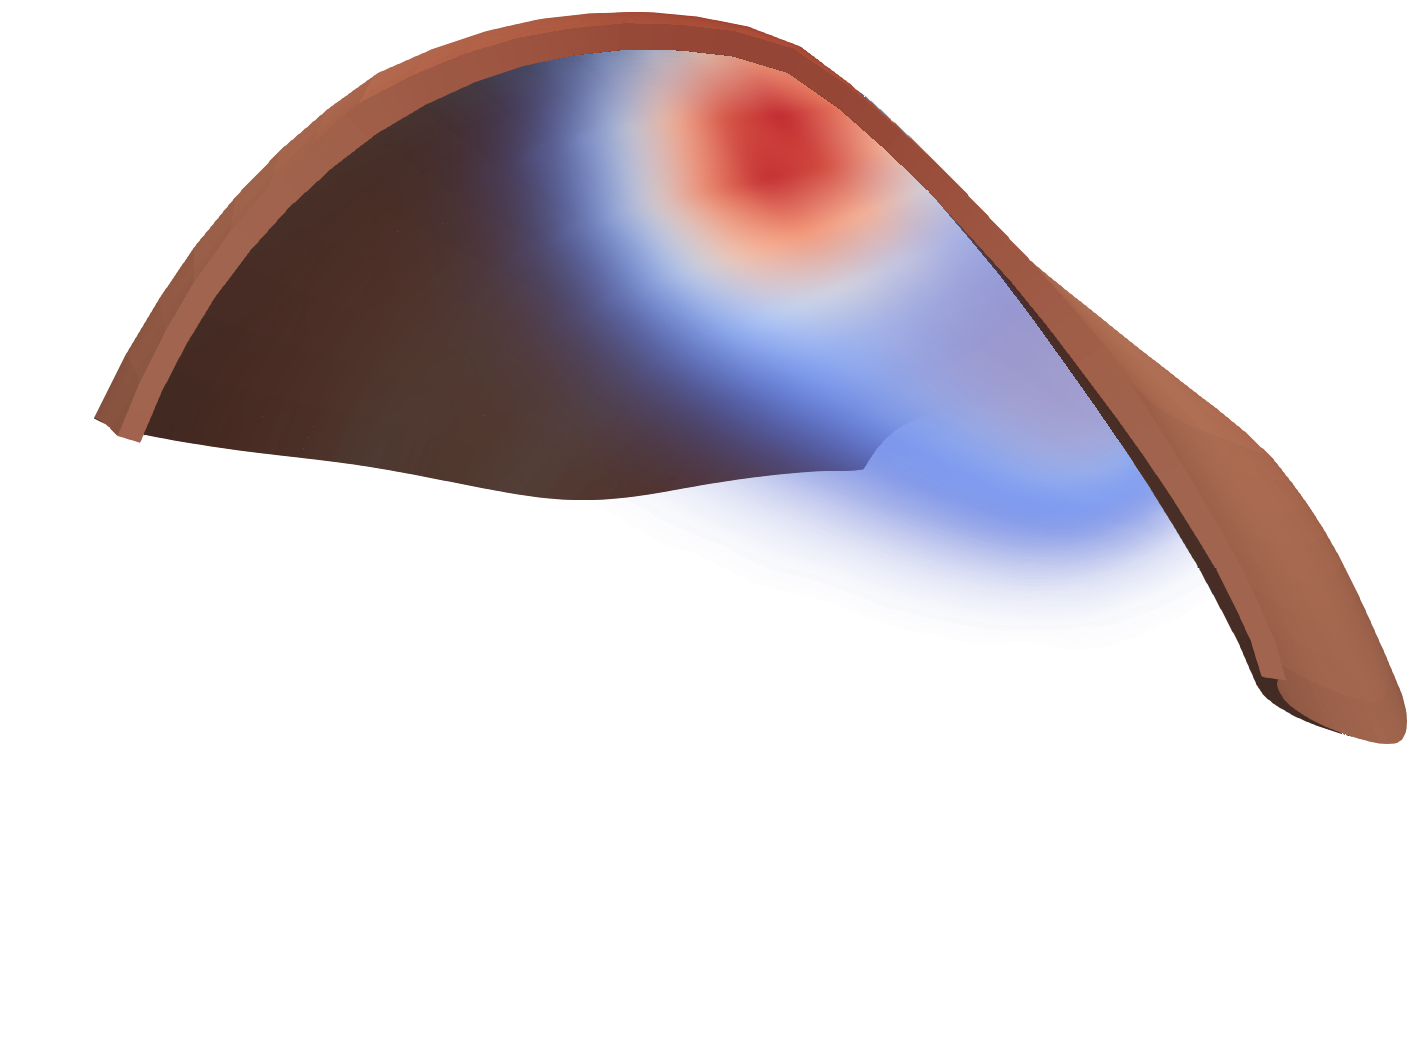
\includegraphics[width=\textwidth]{images/results/application/multidomain_fr0_cropped.png}%
    \caption{$f_r^1$}%
    \label{fig:fr0}%
  \end{subfigure}
  \,
  \begin{subfigure}[t]{0.23\textwidth}%
    \centering%
    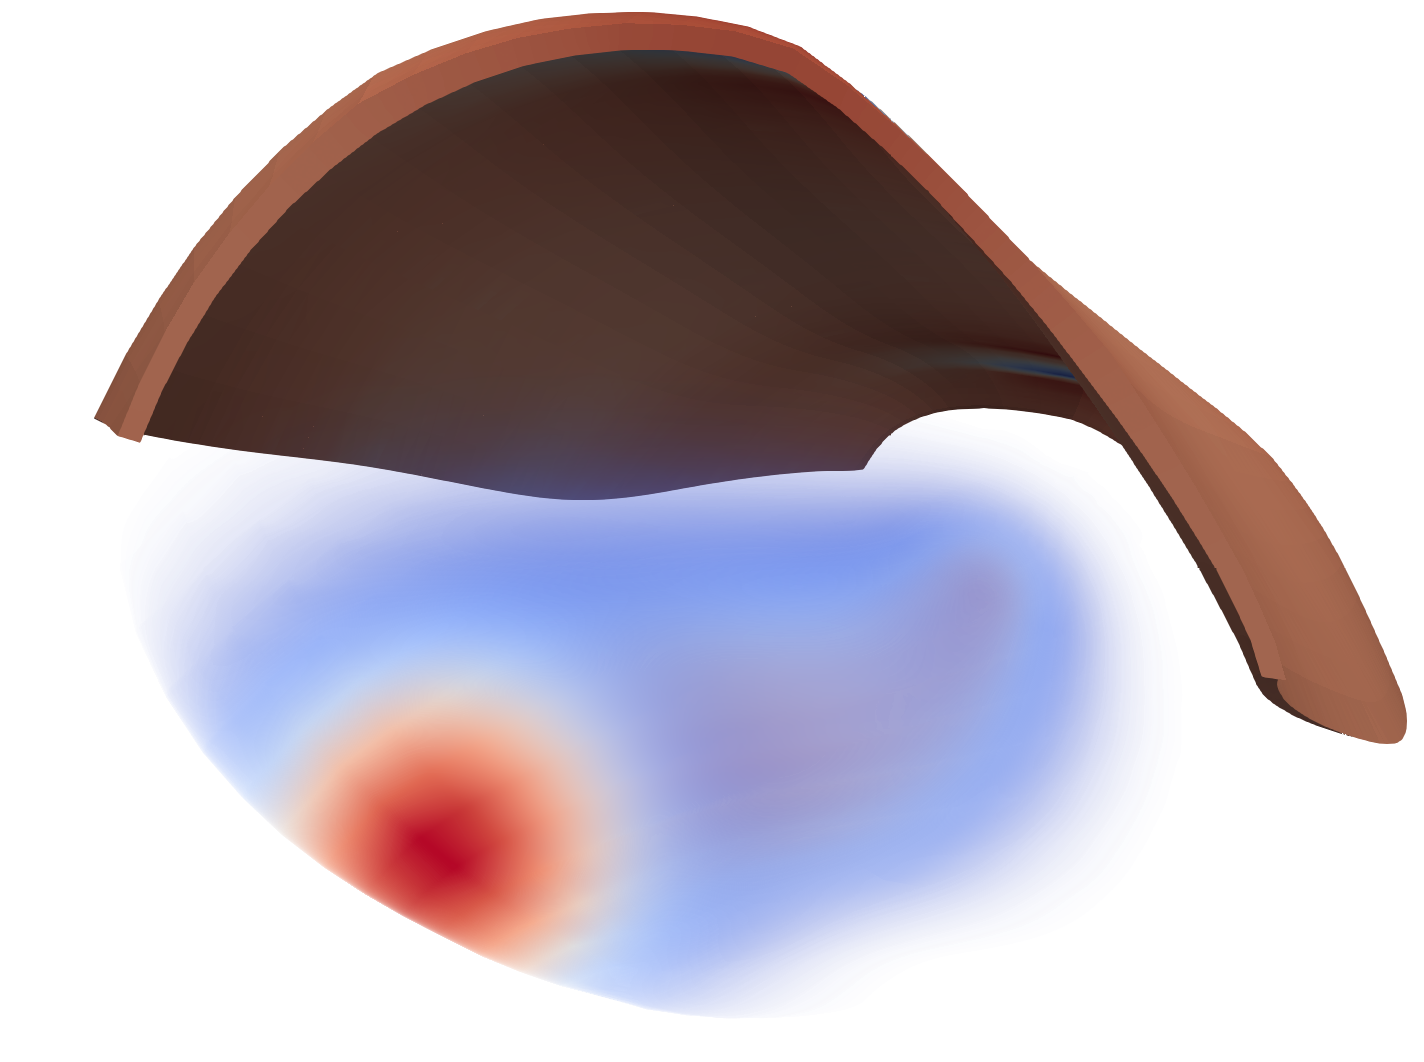
\includegraphics[width=\textwidth]{images/results/application/multidomain_fr1_cropped.png}%
    \caption{$f_r^2$}%
    \label{fig:fr1}%
  \end{subfigure}
  \,
  \begin{subfigure}[t]{0.23\textwidth}%
    \centering%
    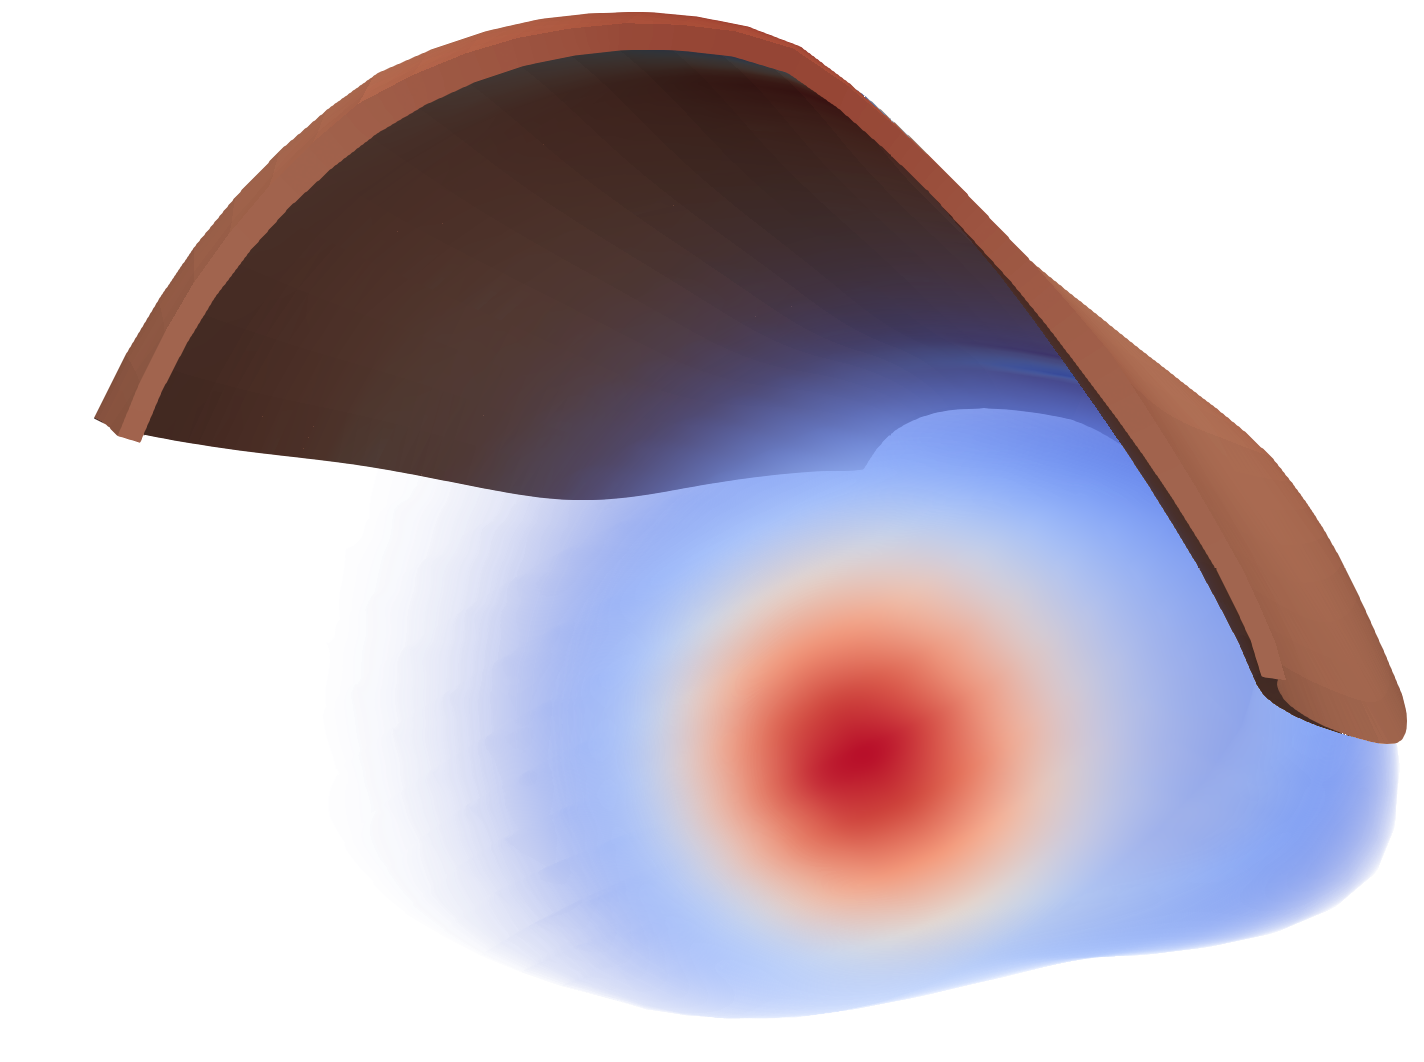
\includegraphics[width=\textwidth]{images/results/application/multidomain_fr2_cropped.png}%
    \caption{$f_r^3$}%
    \label{fig:fr2}%
  \end{subfigure}
  \,
  \begin{subfigure}[t]{0.23\textwidth}%
    \centering%
    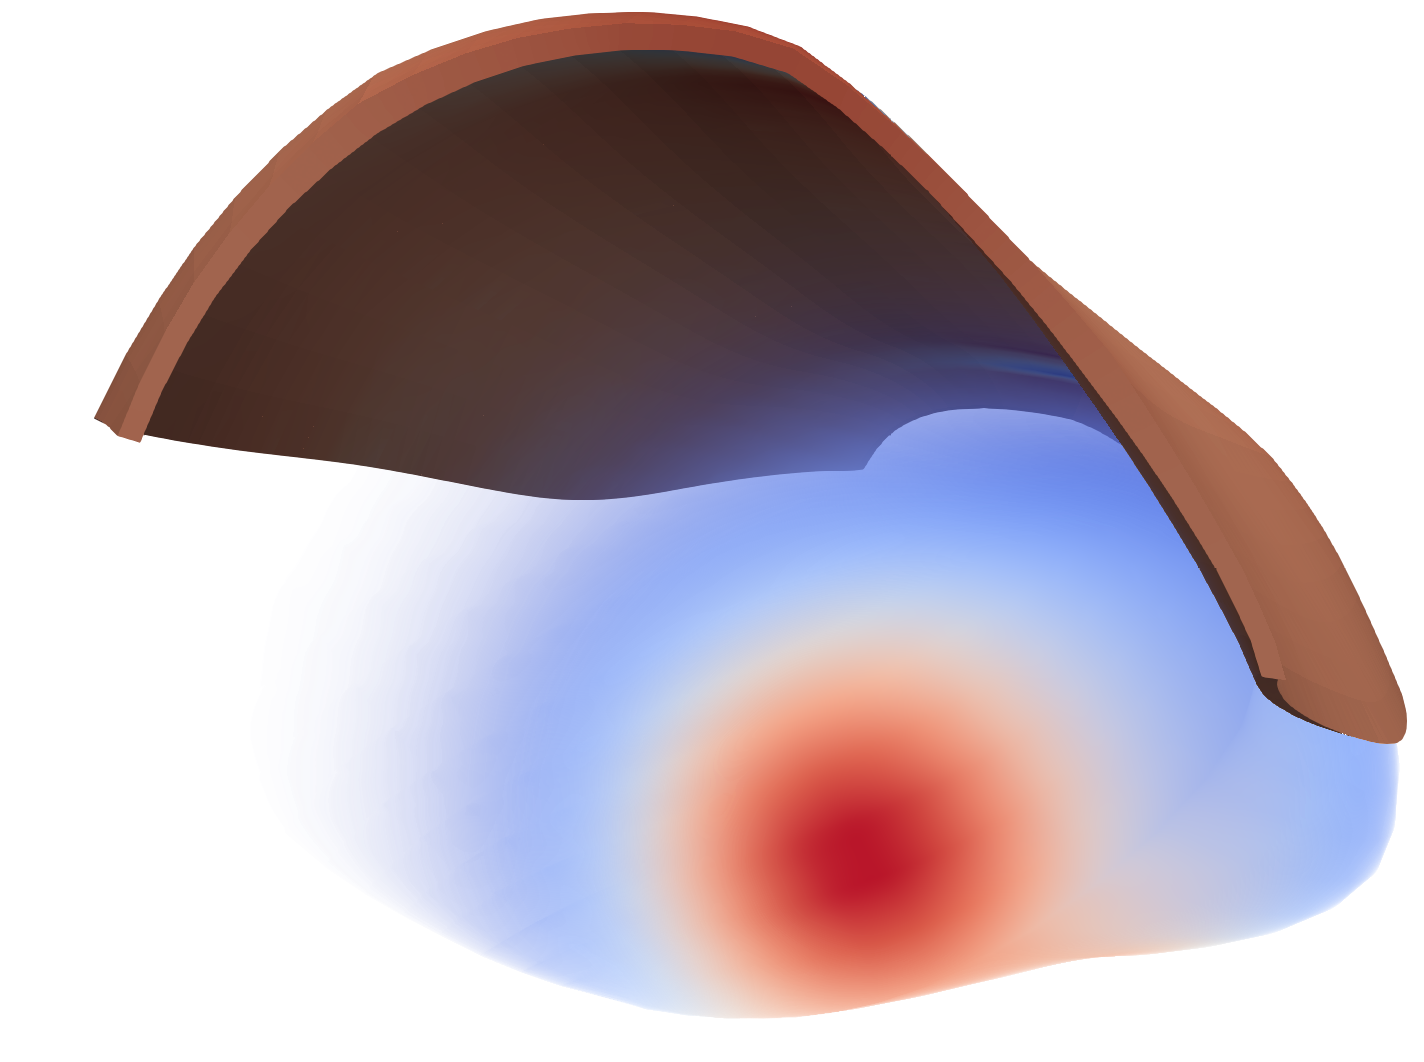
\includegraphics[width=\textwidth]{images/results/application/multidomain_fr3_cropped.png}%
    \caption{$f_r^4$}%
    \label{fig:fr3}%
  \end{subfigure}
  \caption{Simulation of electrophysiology with the multidomain model: Value of the occupancy factors $f_r^k$ for MUs 1 to 4. The color coding encodes the maximum value by red color and the decreasing value along the radius by increased transparency and the color transition to blue color. The locations where the factor vanishes, $f_r^k=0$, correspond to full transparency.}%
  \label{fig:multidomain_fr}%
\end{figure}%

\Cref{fig:multidomain_fr} shows the MU occupancy factors for the four MUs in the considered example scenario. It can be seen that the individual MU territories only occupy a small fraction of the muscle domain and are centered around fibers in longitudinal direction of the muscle.

Results of the simulation at $t=\SI{14}{\ms}$ are given in \cref{fig:multidomain_4mus}. In the considered scenario, the first and second MU are stimulated at $t=\SI{0}{\ms}$ and $t=\SI{10}{\ms}$, respectively. At the time of the displayed images, MUs 3 and 4 have not yet been stimulated. 

Upon stimulation, we prescribe the membrane voltage $V_m$ for one timestep as $\SI{20}{\milli\volt}$ at the stimulated nodes in the mesh of the respective MU. In this scenario, the stimulated nodes are located in the middle of the muscle in longitudinal direction in three adjacent cross-sectional layers of mesh elements.

The upper two images in \cref{fig:multidomain_4mus} show the locations of the propagated action potential fronts at $t=\SI{14}{\ms}$ for MU 1 and MU 2, given by the values of $V_m^k$. While the action potentials span the entire cross-section of the muscle domain, they contribute to the EMG value scaled by their locally varying occupancy factor $f_r^k$.

% multidomain Vm MUs
\begin{figure}
  \centering%
  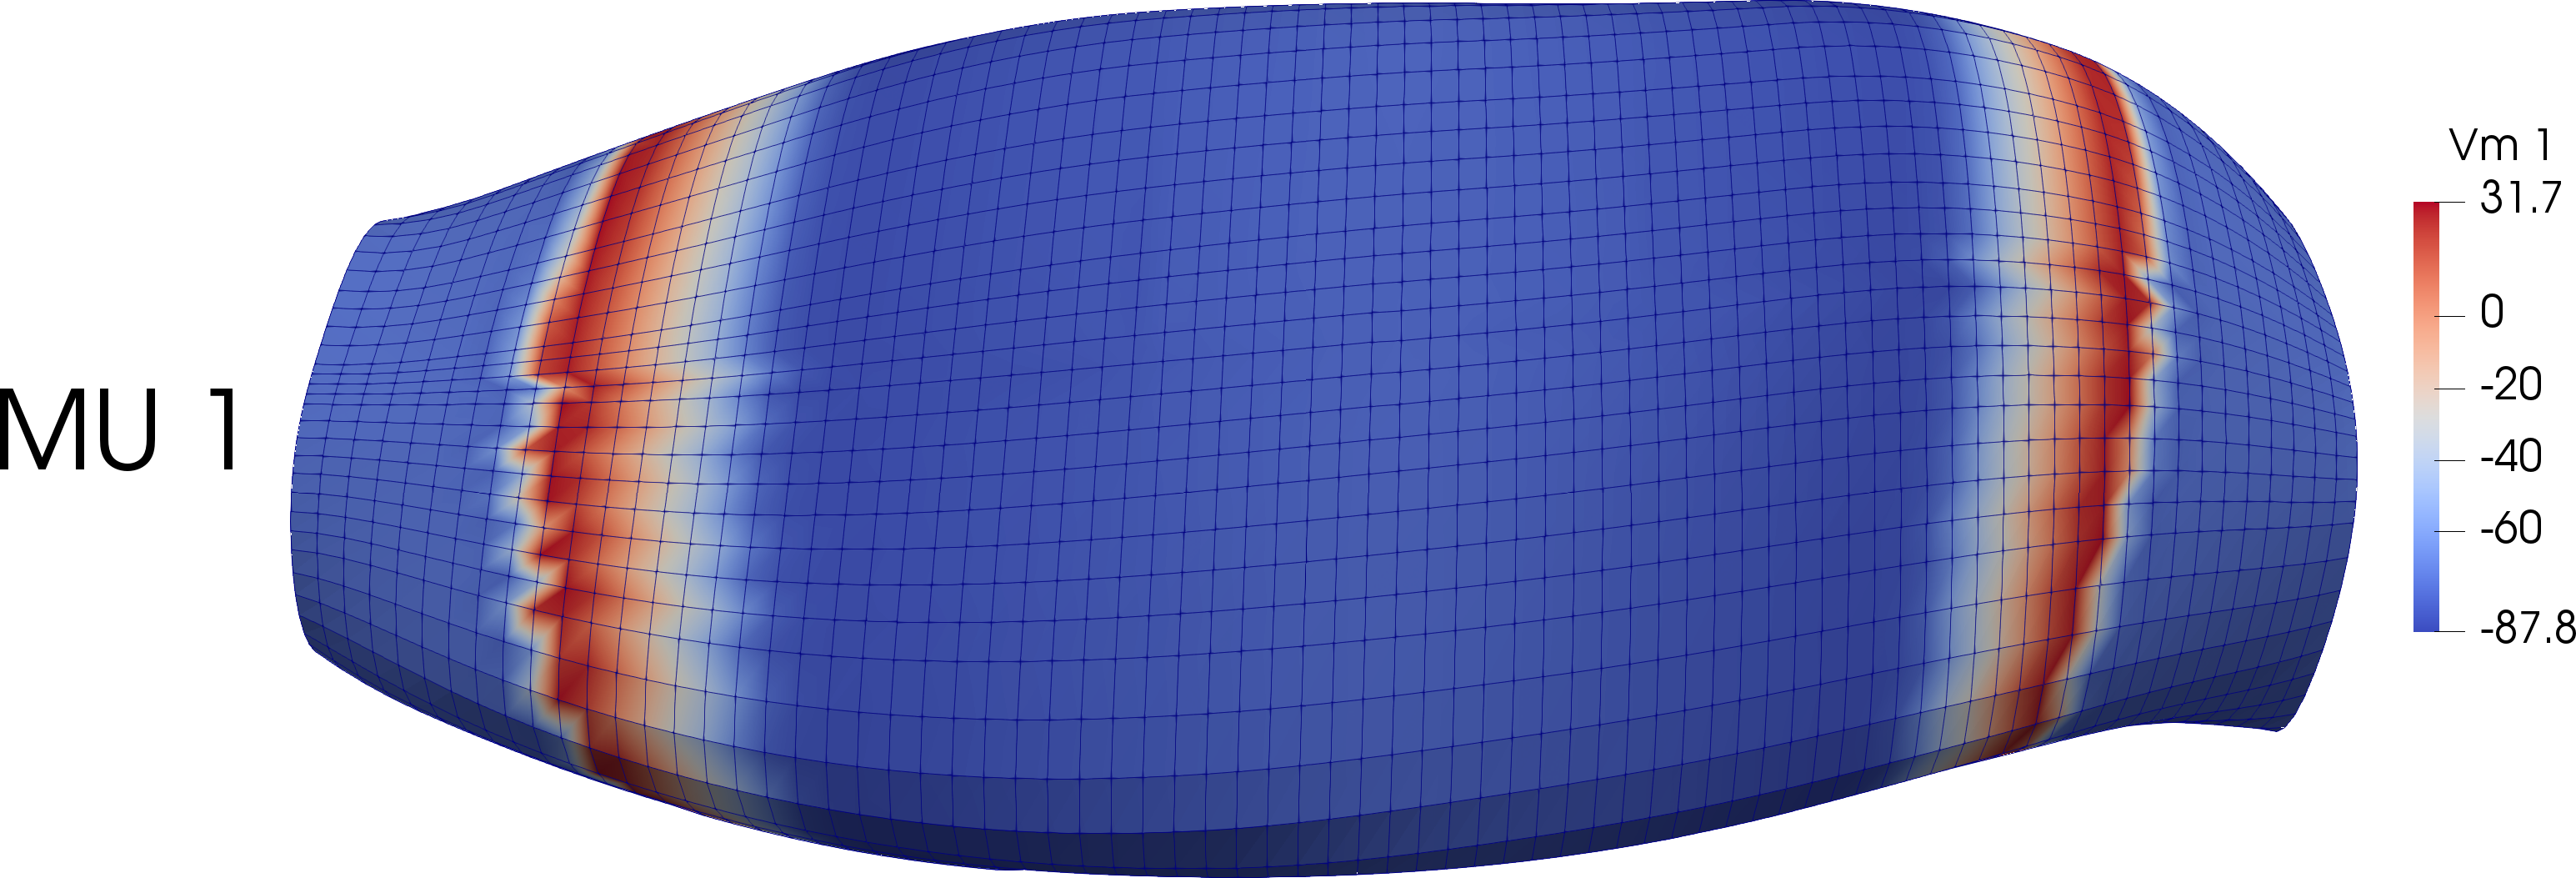
\includegraphics[width=\textwidth]{images/results/application/multidomain_4mus_mu1.png}\\[4mm]
  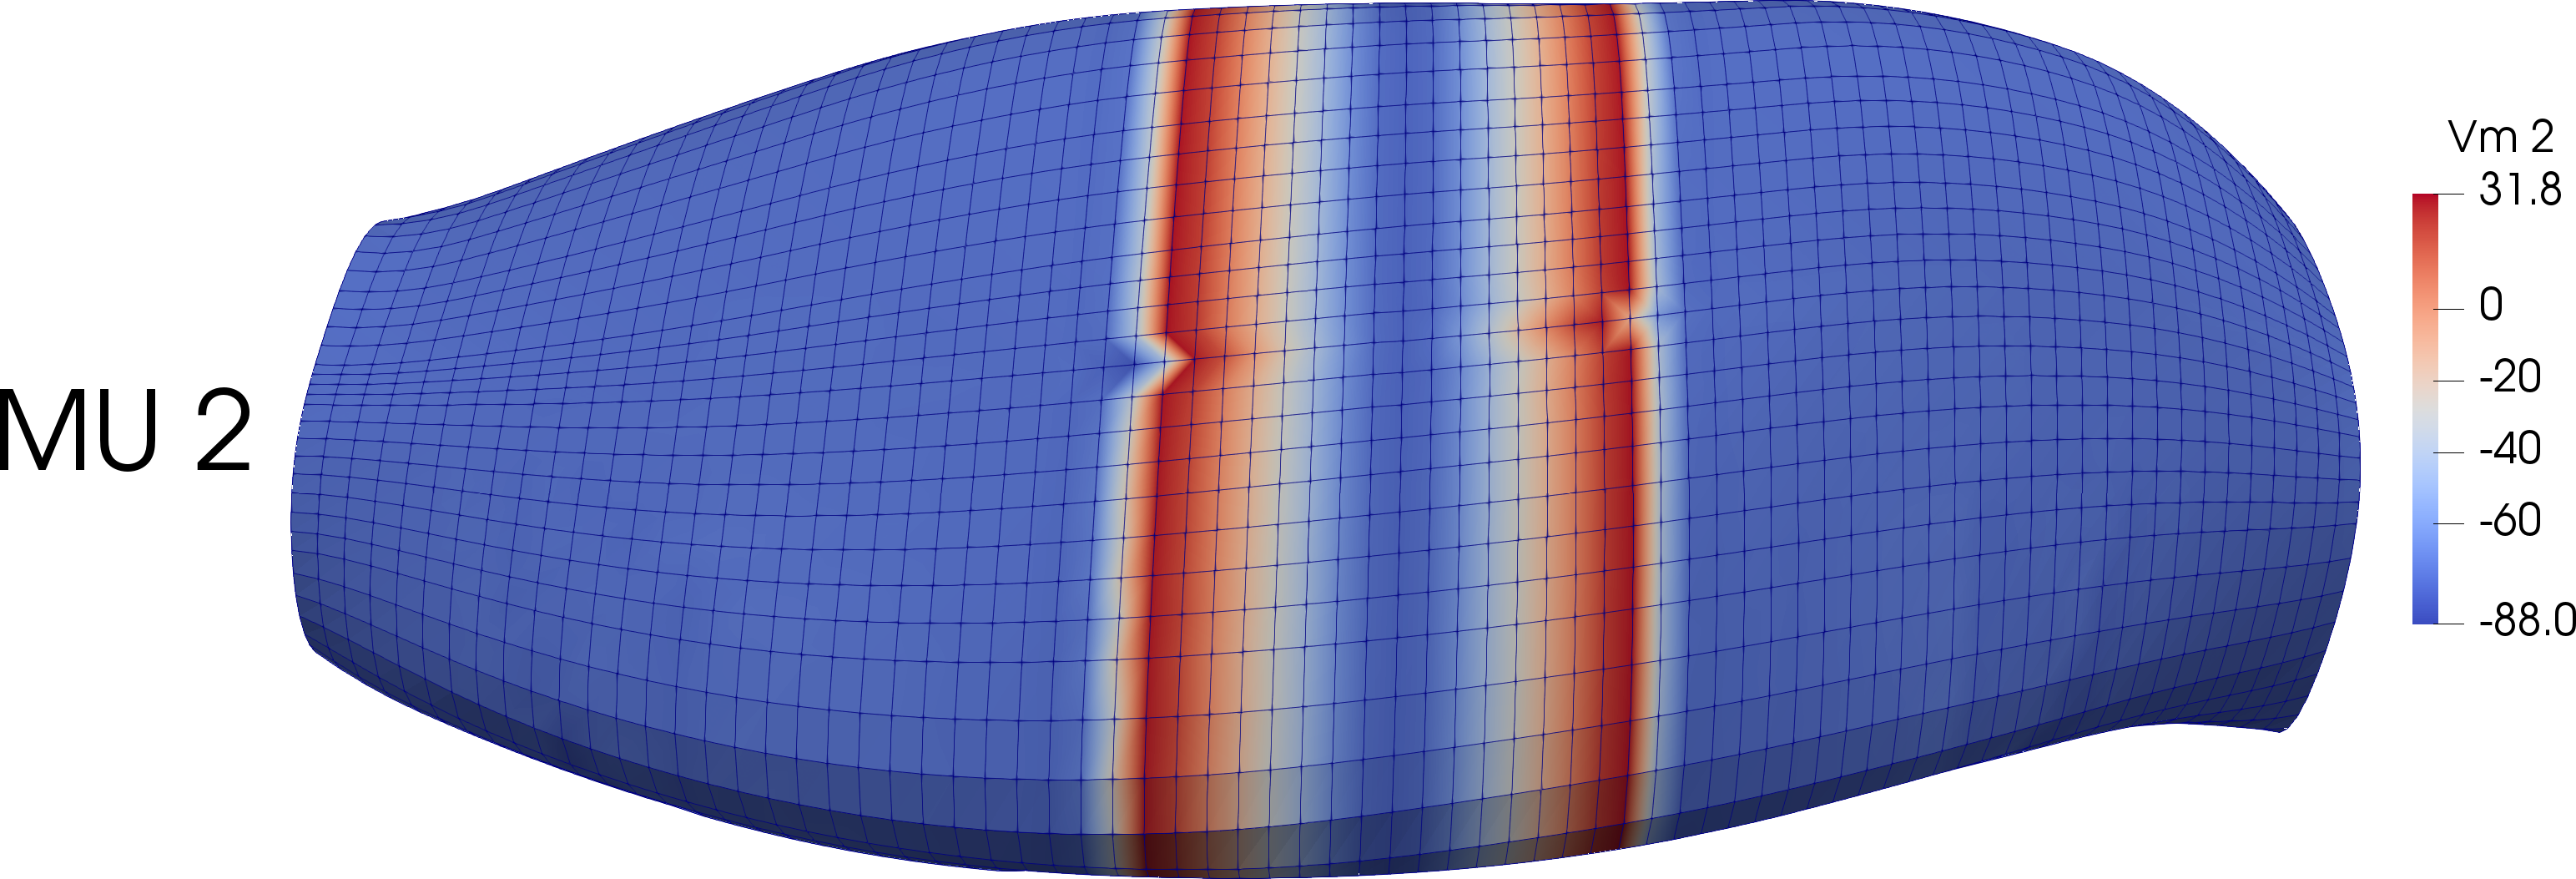
\includegraphics[width=\textwidth]{images/results/application/multidomain_4mus_mu2.png}\\[4mm]
  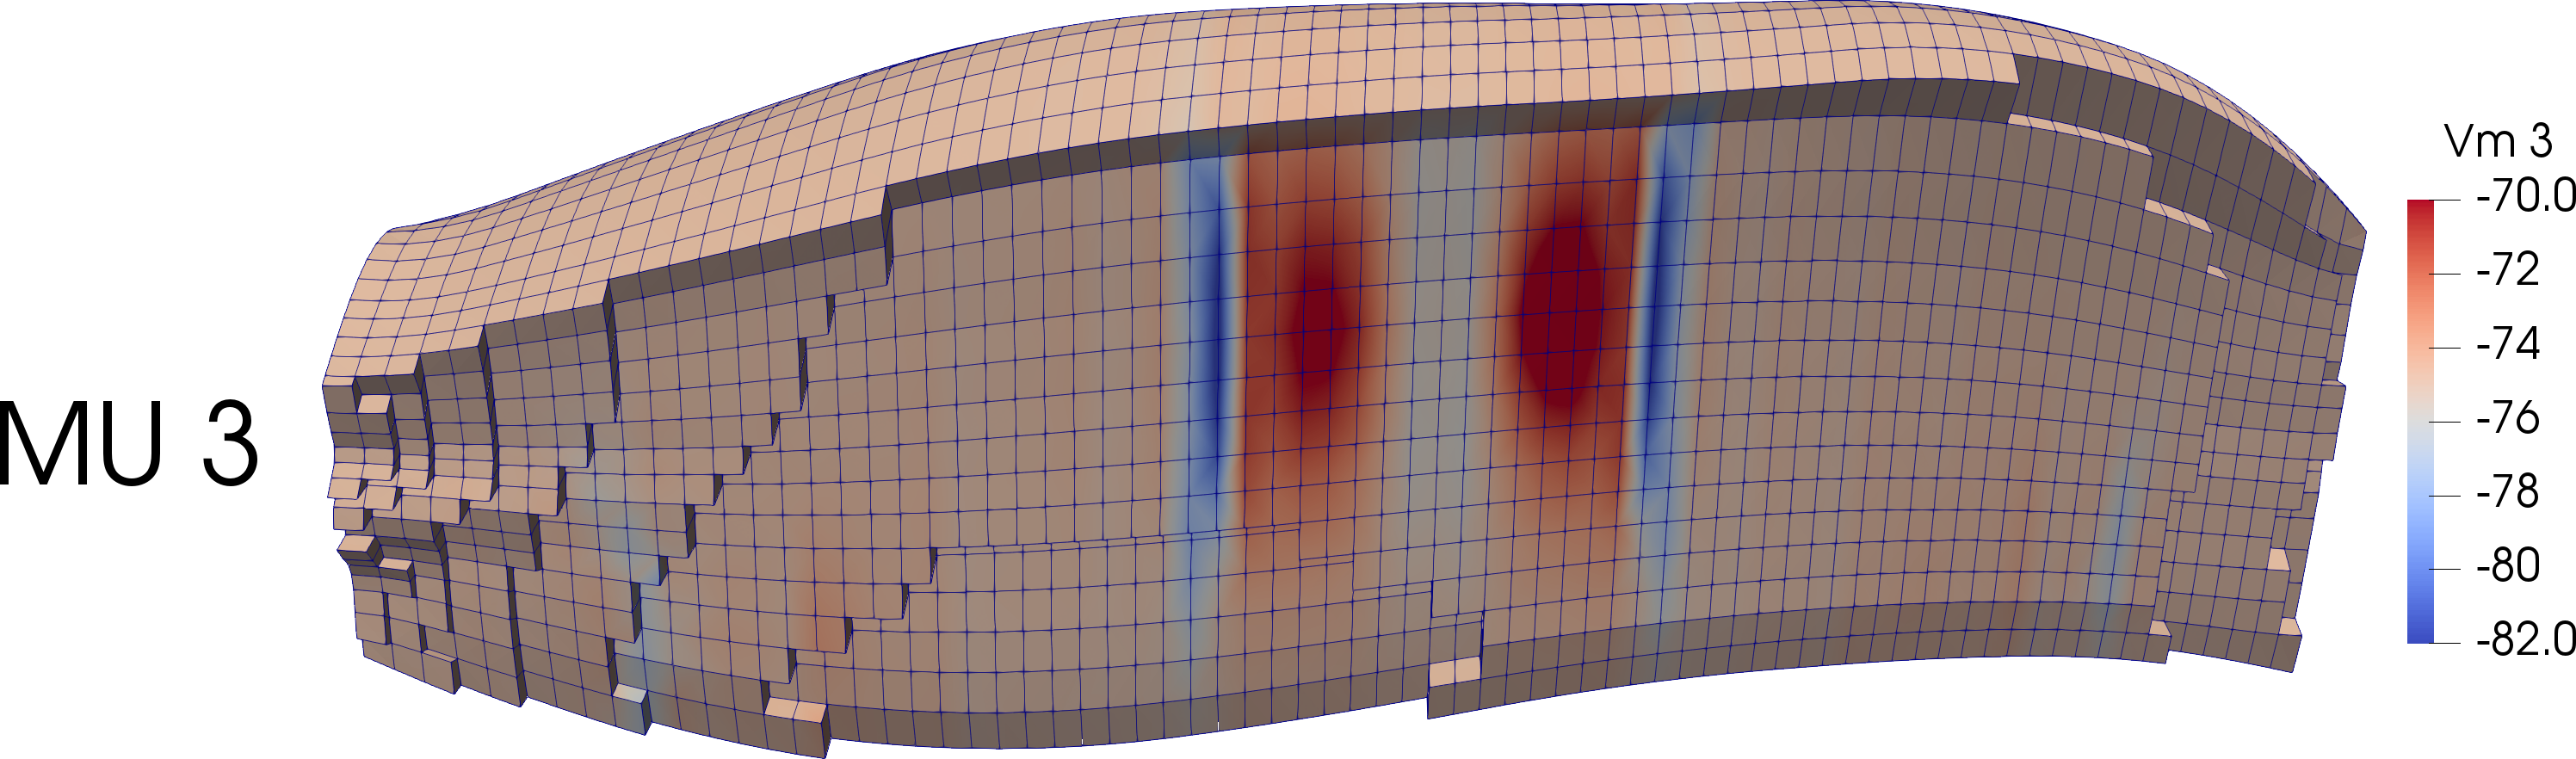
\includegraphics[width=\textwidth]{images/results/application/multidomain_4mus_mu3.png}\\[4mm]
  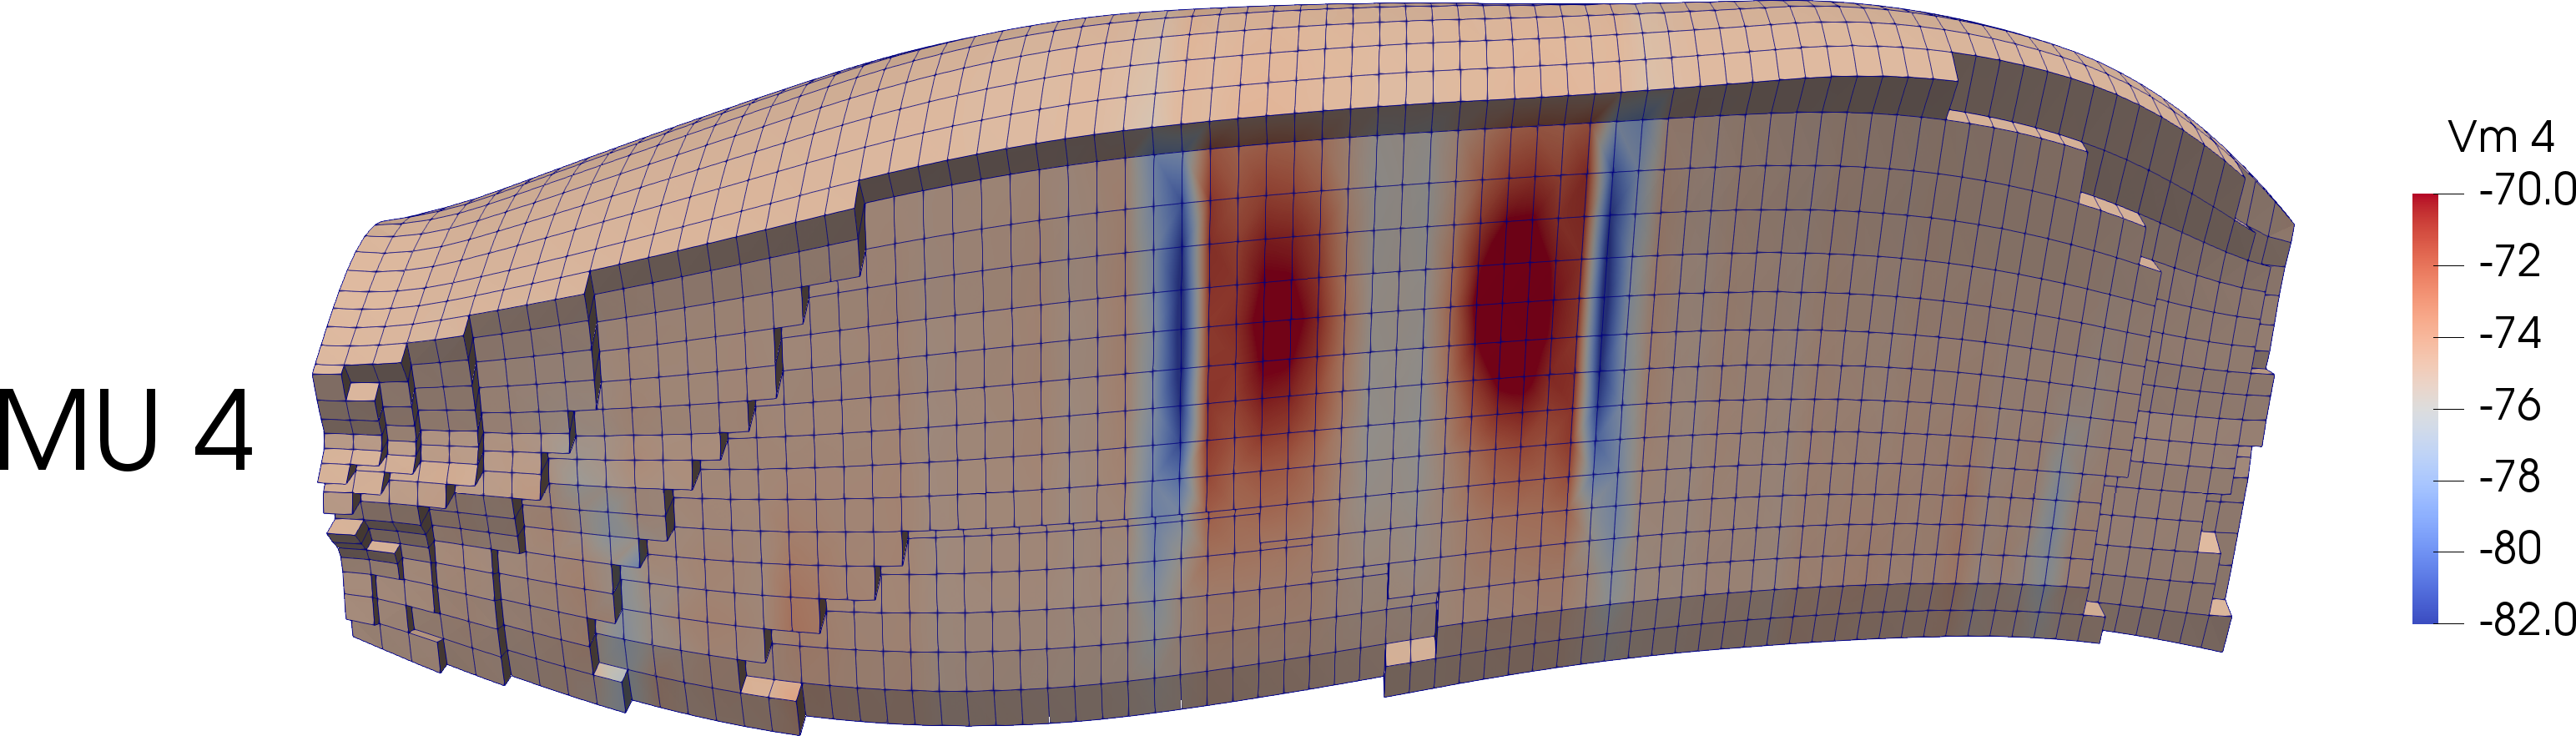
\includegraphics[width=\textwidth]{images/results/application/multidomain_4mus_mu4.png}%
  \caption{Simulation of electrophysiology with the multidomain model: Transmembrane potential $V_m^k$ of MUs 1 to 4 at $t=\SI{14}{\ms}$.}%
  \label{fig:multidomain_4mus}%
\end{figure}%

As the $V_m^k$ values of all MUs $k\in \{1,\dots,N_\text{MU}\}$ are strongly coupled, the active MUs, MU 1 and MU 2, influence the $V_m^k$ scalar fields of the inactive MUs, MU 3 and MU 4. The lower two images in \cref{fig:multidomain_4mus} show the computational domain of the muscle with several layers of 3D elements removed. 
It can be seen that, at some regions in the interior of the domain, the values of $V_m^3$ and $V_m^4$ correspond to the negated value of $V_m^2$ with a smaller absolute value. Note the different color scales for $V_m^1$, $V_m^3$ and $V_m^4$ in these images.

\Cref{fig:multidomain_4mus_body} shows the values of the extracellular potential $\phi_e$ on the muscle domain. The contributions from the two active MUs can be seen. 
\Cref{fig:multidomain_4mus_phi_e_points} gives an impression of the used mesh and shows the value of $\phi_e$ for all nodes. It can be seen that the $\phi_e$ values span a larger value range in the interior of the domain than on the boundary, as previously shown in \cref{fig:multidomain_4mus_body}. Correspondingly, the color coding in \cref{fig:multidomain_4mus_phi_e_points} uses a larger range than in \cref{fig:multidomain_4mus_body}.

\Cref{fig:multidomain_4mus_emg} shows the EMG values $\phi_b$ on the surface of the body domain mesh. The effect of the body domain is revealed by comparing the electric potential on the boundary of the muscle mesh in \cref{fig:multidomain_4mus_body} with the values in \cref{fig:multidomain_4mus_emg}. The signals get locally smoothed by the fat layer.


% multidomain phi_e
\begin{figure}
  \centering%
  \begin{subfigure}[t]{\textwidth}%
    \centering%
    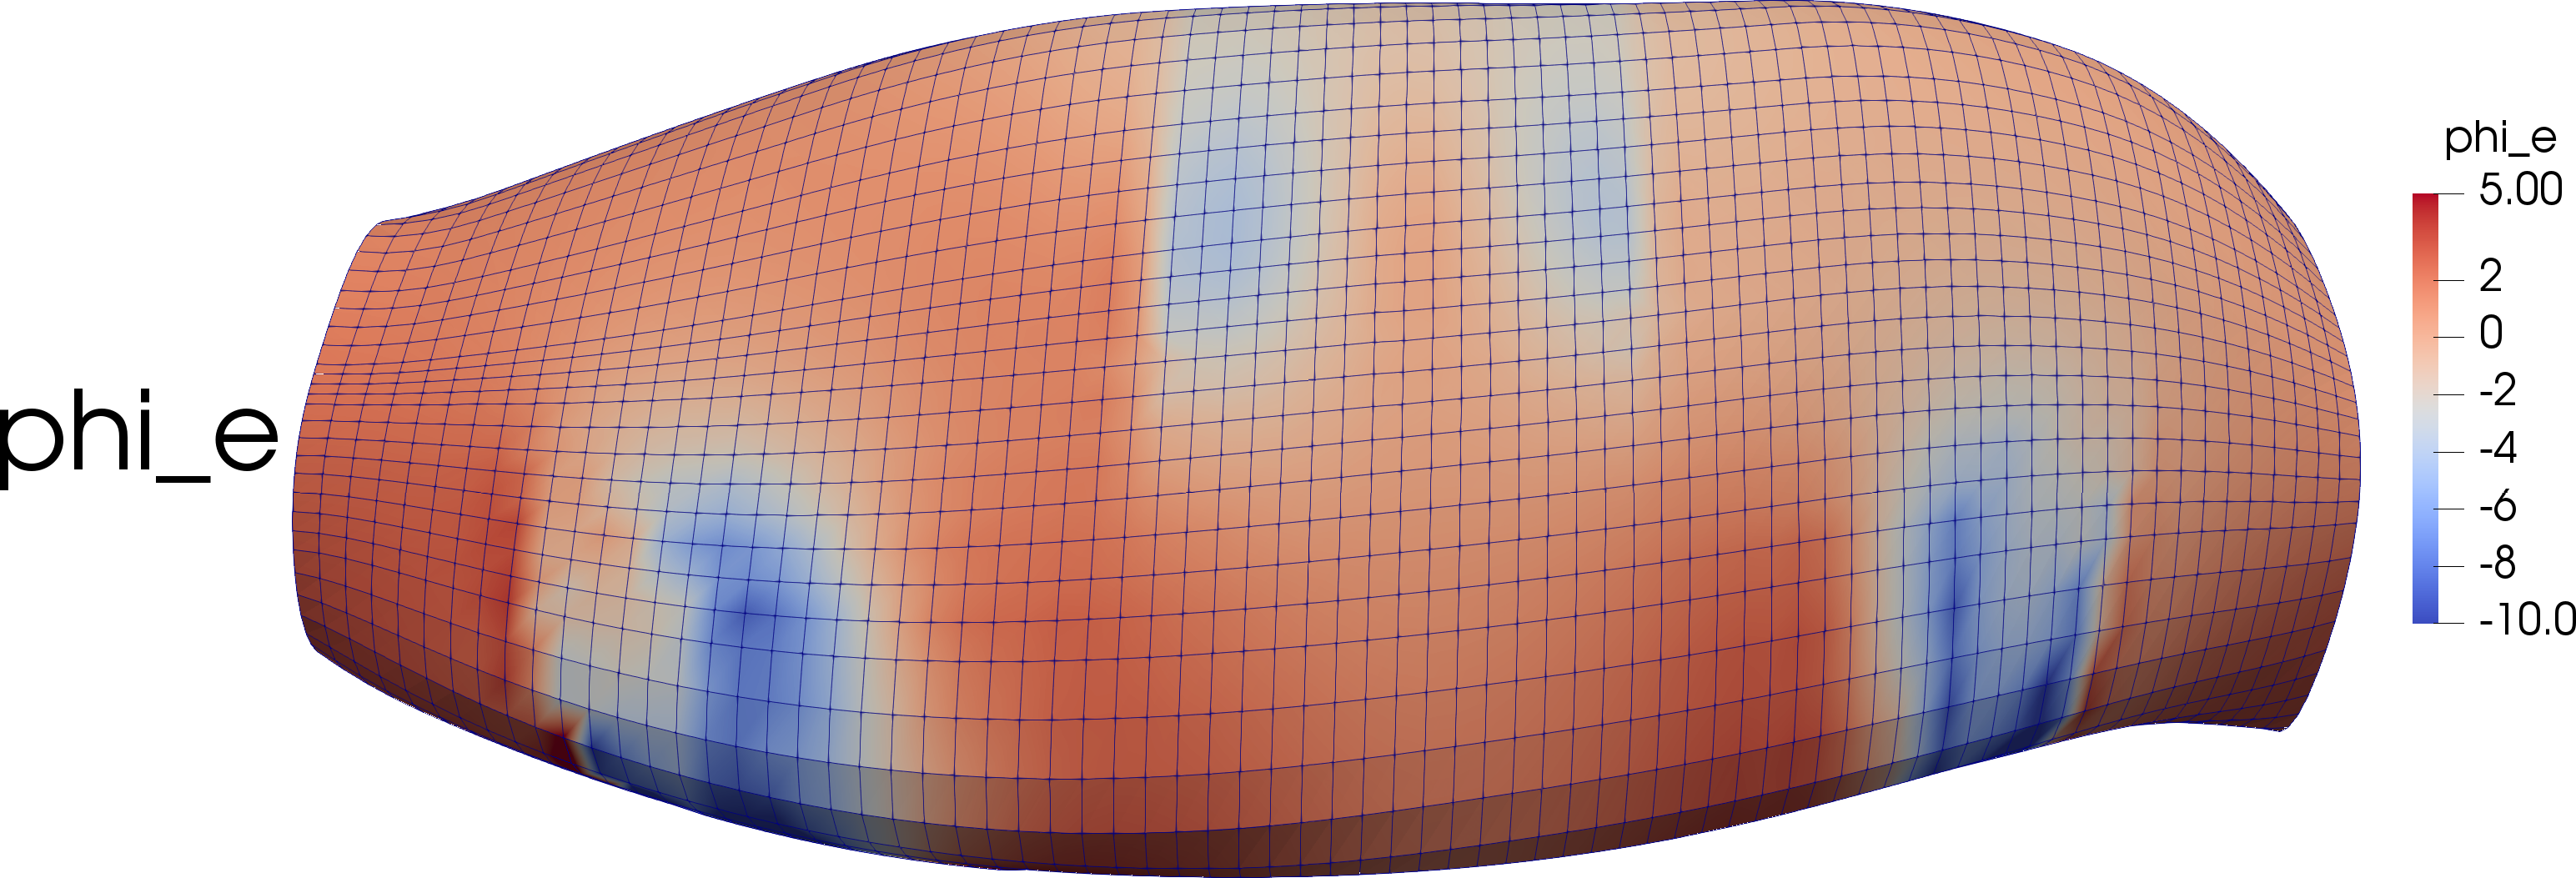
\includegraphics[width=\textwidth]{images/results/application/multidomain_4mus_body.png}%
    \caption{Extracellular potential $\phi_e$ on the surface of the muscle domain.}%
    \label{fig:multidomain_4mus_body}%
  \end{subfigure} \\
  \begin{subfigure}[t]{\textwidth}%
    \centering%
    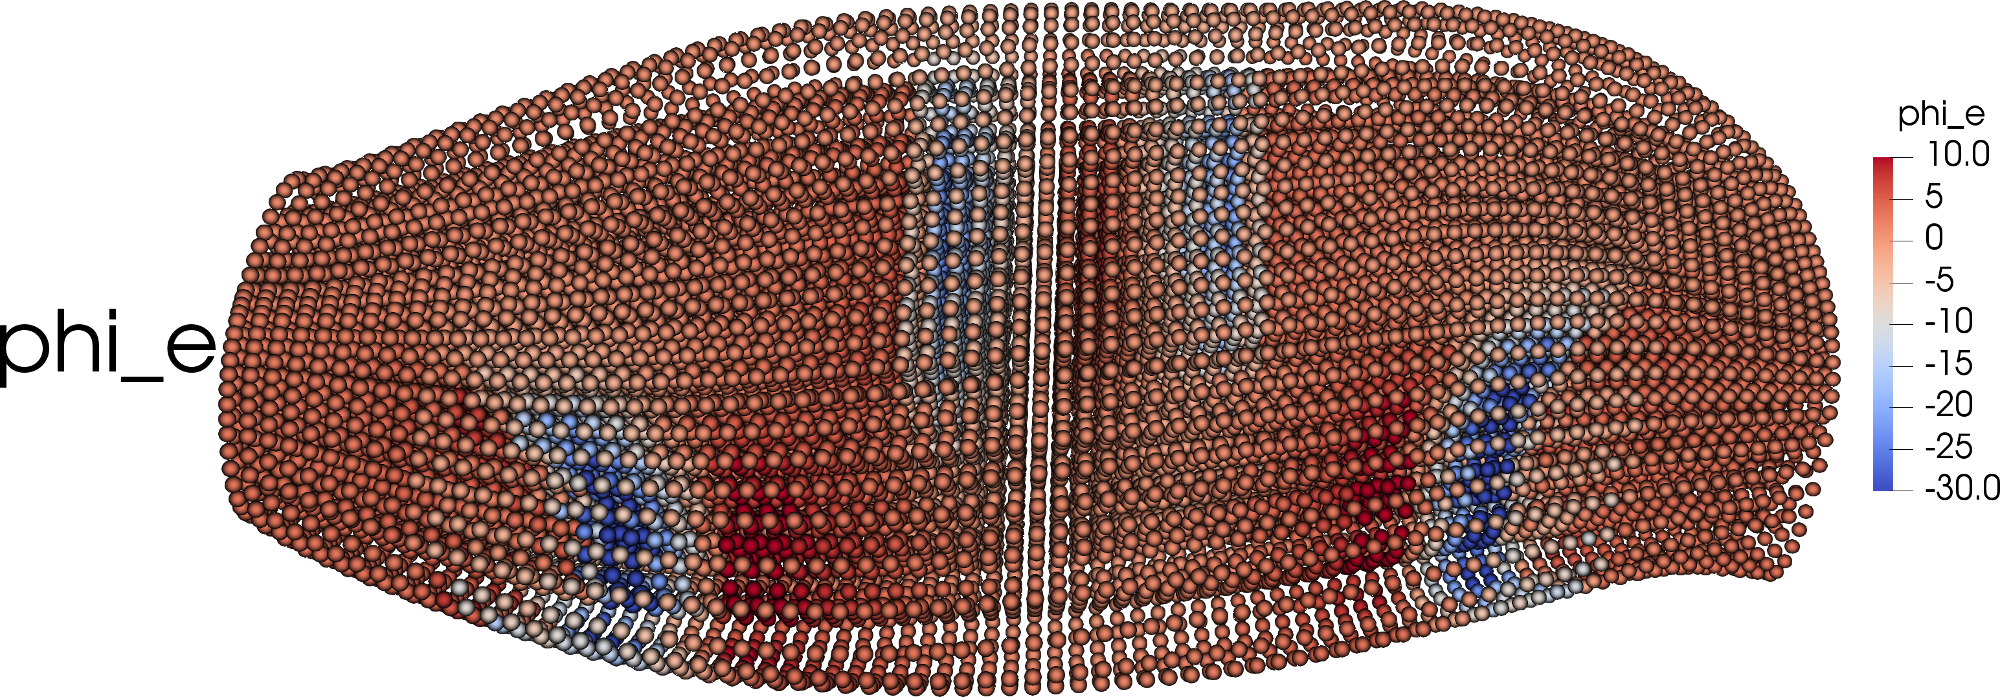
\includegraphics[width=\textwidth]{images/results/application/multidomain_4mus_phi_e_points.png}%
    \caption{Extracellular potential $\phi_e$ at points of the 3D muscle mesh.}%
    \label{fig:multidomain_4mus_phi_e_points}%
  \end{subfigure} \\
  \begin{subfigure}[t]{\textwidth}%
    \centering%
    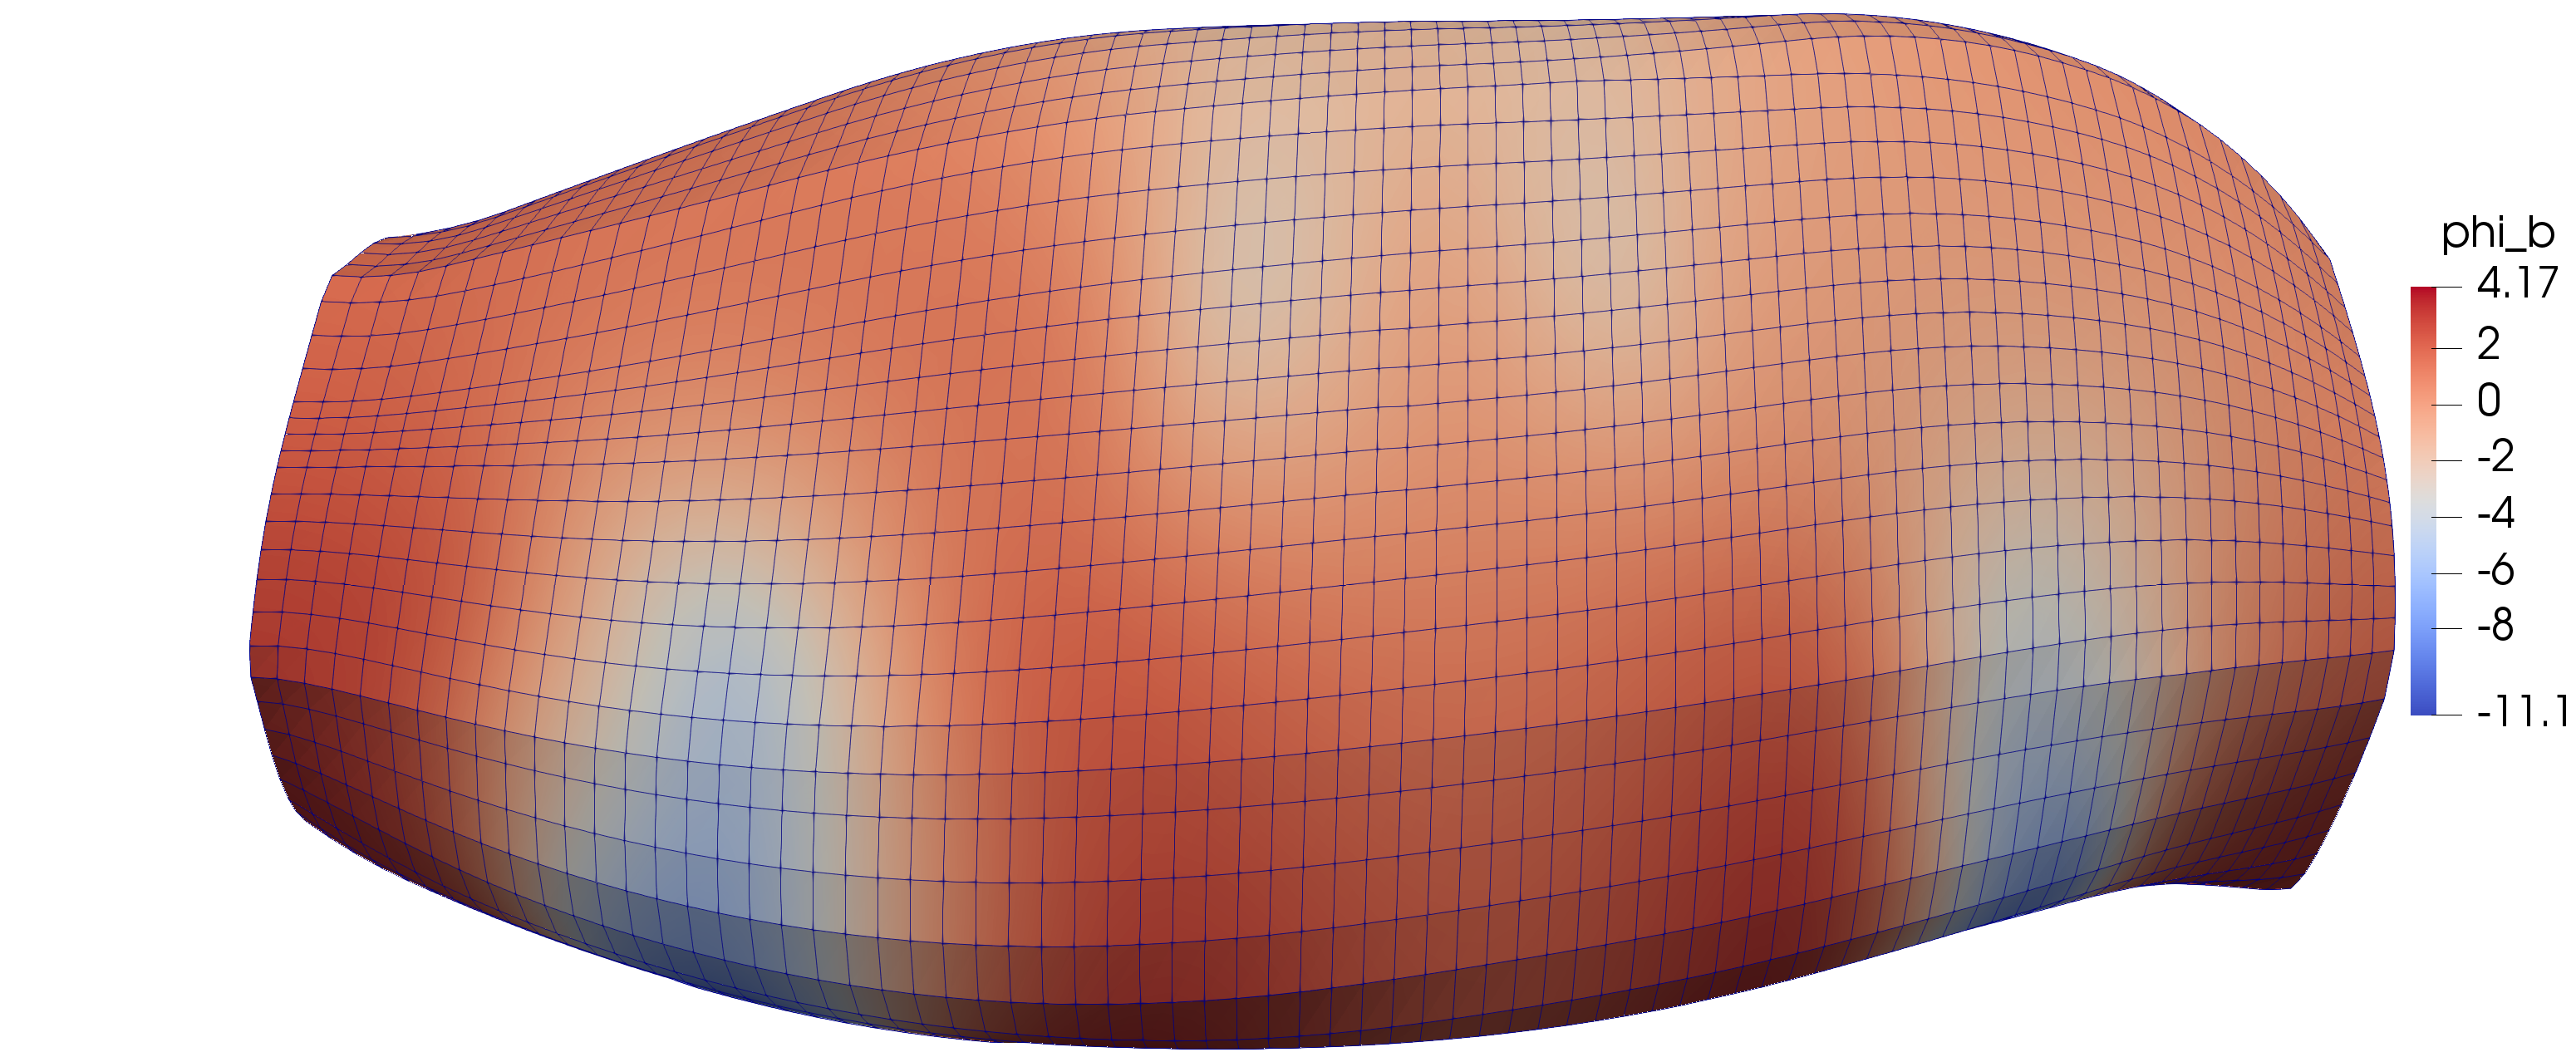
\includegraphics[width=\textwidth]{images/results/application/multidomain_4mus_emg.png}%
    \caption{EMG signal $\phi_b$ on the surface of the body fat domain. The comparison with (a) shows the effect of the fat layer.}%
    \label{fig:multidomain_4mus_emg}%
  \end{subfigure}
  \caption{Simulation of electrophysiology with the multidomain model: Simulation results at $t=\SI{14}{\ms}$ for a scenario with 4 MUs.}%
  \label{fig:multidomain_4mus_2}%
\end{figure}%



\subsection{Simulation of EMG Signals}\label{sec:multidomain_simulation_emg}

In the second scenario, we simulate a higher number of 25 MUs. The MUs are activated at random times within the first \SI{20}{\ms}. We use a mesh with $12 \times 12 \times 74 = \num{10656}$ elements in the muscle domain and $24 \times 4 \times 74 = 7104$ elements in the body domain. Compared to the mesh in the previous scenario, the spatial resolution in radial direction is chosen slightly coarser, to speed up the computation.
The other model parameters, discretization schemes and solvers are chosen as before.

In this scenario, the stimulated nodes are no longer located in the middle of the muscle, but randomly varied by up to \SI{10}{\percent} of the muscle length using a uniform distribution. This approach to model the neuromuscular junctions is analog to the approach in \cref{sec:simfiber_mu} for the fiber based electrophysiology. 
\Cref{fig:multidomain_25mus_snapshot} shows the membrane voltage $V_m^1$ of MU 1 shortly after the MU has been activated. Because of the different locations of the stimulated points, no uniform action potential \say{front} as in \cref{fig:multidomain_4mus} is seen. Instead, a characteristic 2D MU action potential forms. 

The spike of the depolarized membrane voltage at every stimulated point propagates along the fiber direction and additionally diffuses in  transverse direction. This yields the cone-like structures of lower $V_m$ values as  seen in \cref{fig:multidomain_25mus_snapshot}. The origin of the transverse propagation is the electric conduction in the extracellular space, which is governed by the isotropic conduction tensor $\bfsigma_e$ in \cref{eq:multidomain_isotropic_e}. This isotropic conduction is strongly coupled to the directed action potential propagation within every MU compartment.

The resulting EMG values $\phi_e$ on the muscle boundary and $\phi_b$ on the skin surface are given in \cref{fig:multidomain_25mus2_emg} and \cref{fig:multidomain_25mus2_body}, respectively. The fat layer again smooths out the signal, as observed in the last section and in \cref{sec:simfiber_fat} for the fiber based electrophysiology model.

The two blue vertical stripes in \cref{fig:multidomain_25mus2_emg} with lower $\phi_e$ values correspond to the action potentials of multiple MUs at the respective location. It can be seen that the resulting EMG signal varies more in longitudinal direction than in transverse direction. This can be explained by the wide MU territories in this scenario.

% multidomain Vm MU
% multidomain phi_e
\begin{figure}
  \centering%
  \begin{subfigure}[t]{\textwidth}%
    \centering%
    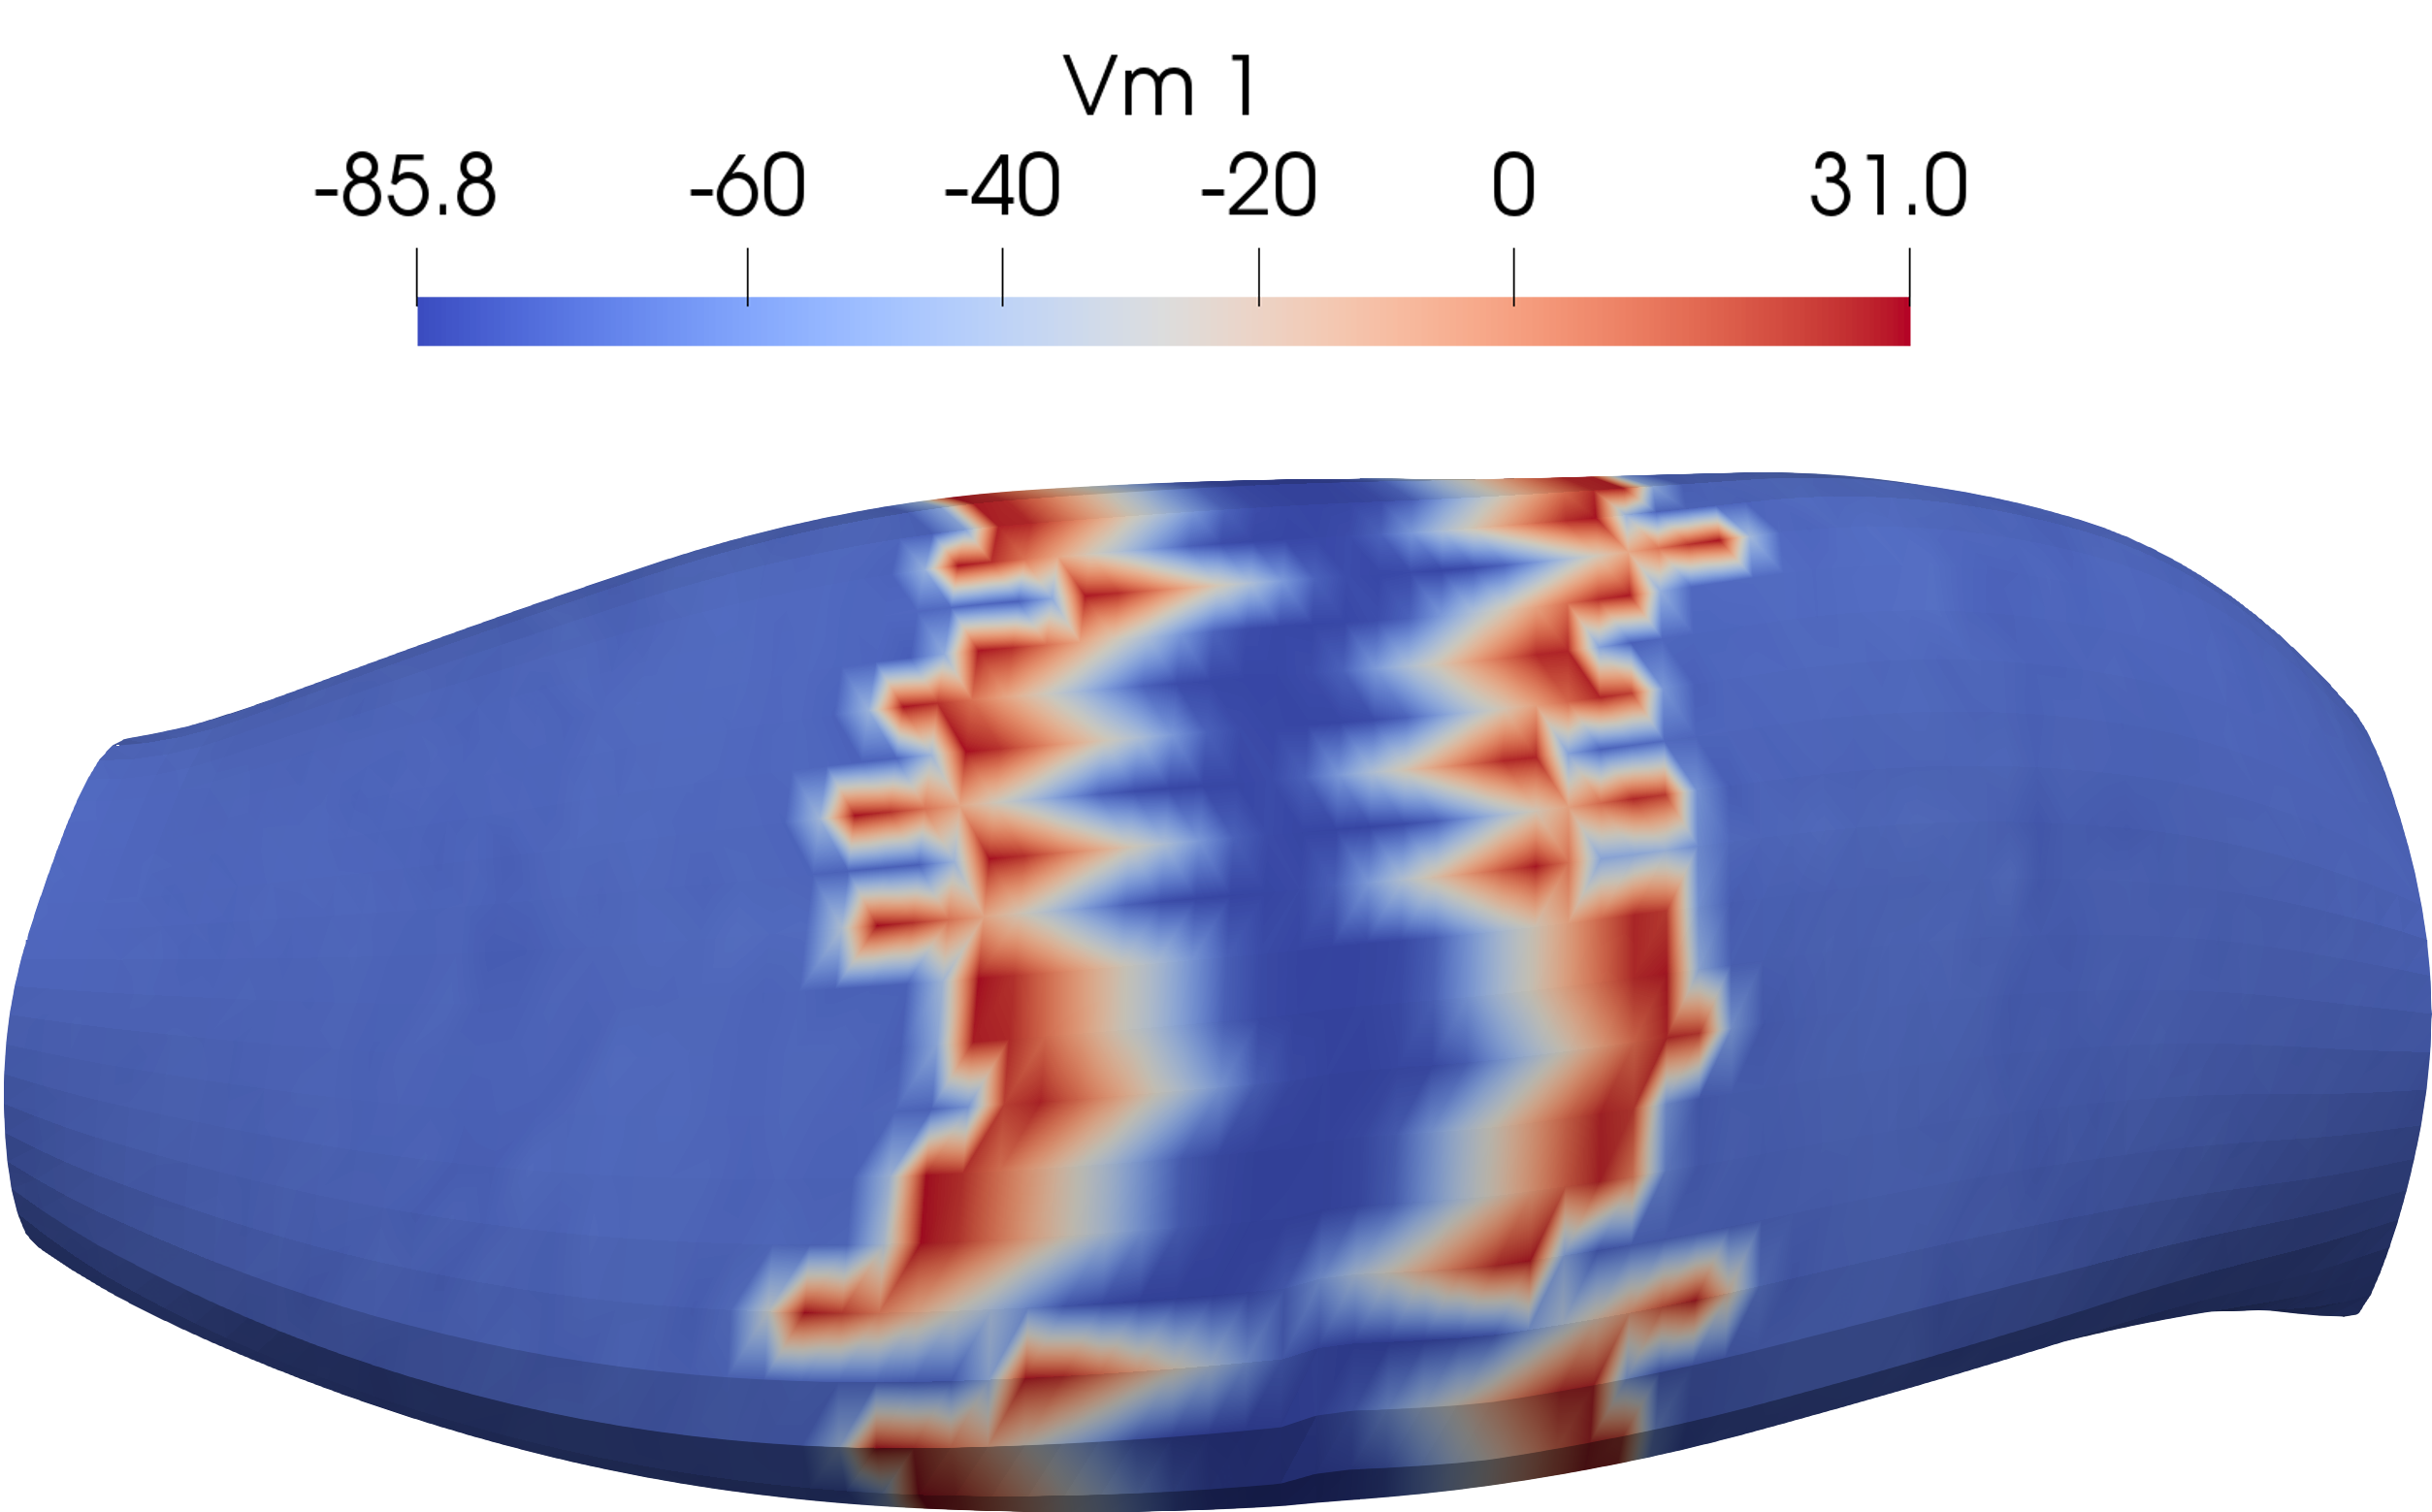
\includegraphics[width=11cm]{images/results/application/multidomain_25mus_snapshot.png}%
    \caption{Transmembrane voltage $V_m^1$ of the first MU.}%
    \label{fig:multidomain_25mus_snapshot}%
  \end{subfigure} \\[4mm]
  \begin{subfigure}[t]{\textwidth}%
    \centering%
    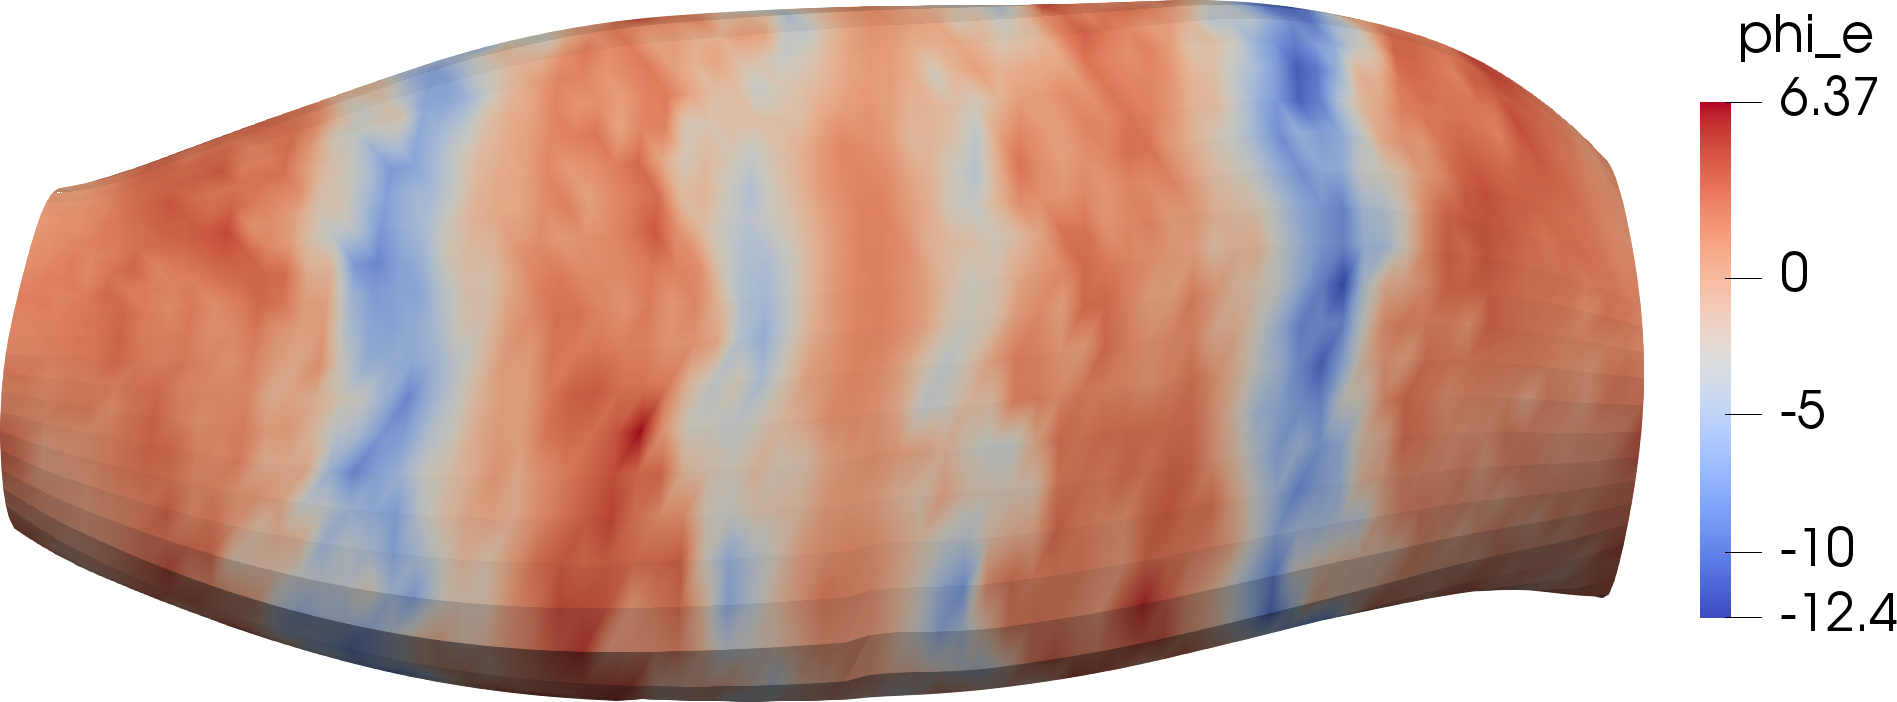
\includegraphics[width=12cm]{images/results/application/multidomain_25mus2_emg.png}%
    \caption{Extracellular potential $\phi_e$ at the surface of the 3D muscle mesh.}%
    \label{fig:multidomain_25mus2_emg}%
  \end{subfigure} \\[4mm]
  \begin{subfigure}[t]{\textwidth}%
    \centering%
    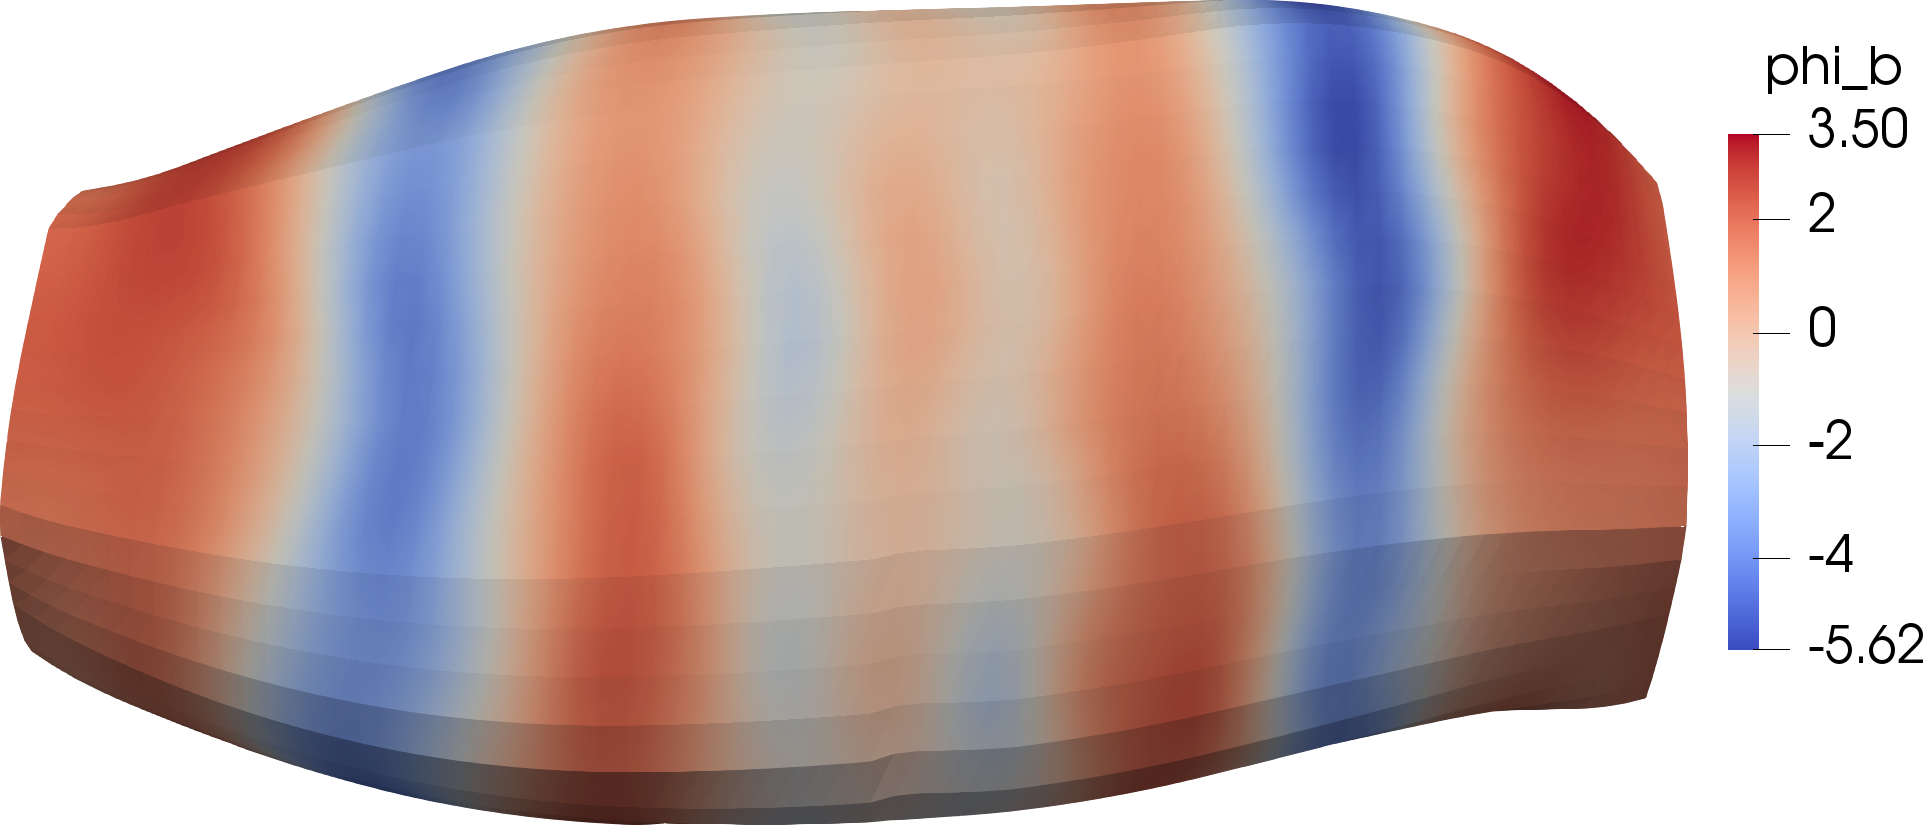
\includegraphics[width=12cm]{images/results/application/multidomain_25mus2_body.png}%
    \caption{EMG signal $\phi_b$ at the surface of the body fat domain.}%
    \label{fig:multidomain_25mus2_body}%
  \end{subfigure}
  \caption{Simulation of electrophysiology with the multidomain model: Simulation results at $t=\SI{20}{\ms}$ for a scenario with 25 MUs.}%
  \label{fig:multidomain_25mus2}%
\end{figure}%


\subsection{Comparison of the Fiber Based Electrophysiology Model and the Multidomain Model}\label{sec:multidomain_differences}

EMG signals on the upper arm can be simulated by both the fiber based electrophysiology model, as demonstrated in \cref{sec:results_fiber_based_electrophysiology} and by the multidomain model, as shown in the previous sections. The two approaches have several similarities and differences.

Both model approaches have in common that they are based on biophysical principles. They both involve a detailed subcellular model, which describes the biochemical processes on the muscle fiber membranes. The subcellular model is solved at discrete points in the 3D domain and the model instances are coupled to a description of electric volume conduction in the muscle domain and the body fat layer.  Both the fiber based approach and the multidomain model are, thus, multi-scale descriptions. 

Both models also resolve the physiological structure of muscle activity given by multiple MUs. Action potential propagation is computed separately for different MUs. In a comprehensive simulation of the neuromuscular system, motor neuron models can be coupled to drive the activation of the MUs.

The two domains of the electrically active muscle tissue and the passive layer of skin and adipose tissue are also considered in both modeling approaches. In the fiber based approach, electric volume conduction is described by the 3D bidomain equation \cref{eq:bidomain1} for the muscle domain and a strongly coupled 3D Laplace equation \cref{eq:body} for the body domain.
The multidomain approach for electric volume conduction generalizes the bidomain model and yields the bidomain equation as a special case, if only one MU is considered. The Laplace equation for the body domain is coupled in the same way as in the fiber based model. In summary, both approaches are very similar regarding the 3D electric conduction part.

The major difference between the models is, that the multidomain approach considers only 3D domains, whereas the fiber based approach resolves individual 1D muscle fibers. Another difference lies in the coupling between the model components. For the fiber based approach, action potential propagation on the 1D fibers is unidirectionally coupled to the 3D volume conduction part of the model. In the multidomain model, all components are bidirectionally coupled. This allows, e.g., to simulate externally applied stimulations by active electrodes on the skin surface. The effects of the external currents on the electric potentials in the 3D muscle volume and down to the 0D subcellular behavior can only be described accurately by the multidomain approach.

The difference in coupling between the action potential propagation model part and the electric volume conduction in the extracellular space can also be seen in the computed EMG signals. A comparison of EMG simulations using the fiber based model, e.g., \cref{fig:emg273529b}, and the multidomain model, e.g., \cref{fig:multidomain_25mus2_emg}, shows that the multidomain approach yields less sharp artifacts in the 2D EMG signal on the muscle surface than the fiber based method. In the fiber based model, the action potentials of individual fibers are visible in the signal. In the multidomain simulations, the regions of similar activity are more clustered in the resulting EMG signals.

Other differences between the two model approaches exist in terms of the computational performance properties of their solvers. In the fiber based approach, action potential propagation can be computed independently for all muscle fibers, which enables large speedups by parallelization and makes large problem sizes with realistic numbers of muscle fibers feasible. For example, \cref{sec:effects_of_the_mesh_width_emg} presents the simulation of \num{270000} muscle fibers with \num{27000} compute cores.
In the multidomain approach, on the other hand, a large linear system of equations has to be solved in every timesteps. This can also be parallelized, but requires communication between the involved processes, which limits the parallel scalability for large problem sizes.

In the multidomain model, the computational effort increases, in good approximation, linearly with both the number of MUs and the number of nodes in the mesh. In the fiber based approach, the amount of computational work mainly corresponds to the number of fibers, not to the number of MUs. 
The 3D problem and, thus, the mesh width of the 3D mesh, typically plays a minor role in the total runtime for the fiber based approach, as the 3D problem is only solved according to the desired EMG sampling frequency. In the multidomain approach, no separate timestep widths can be chosen for the computations of the extracellular and body domain electric potentials, $\phi_e$ and $\phi_b$, as they are computed as a solution of the same linear system of equations.

For example, the computation of \SI{24}{\ms} of the multidomain scenario in \cref{sec:multidomain_simulation_emg} with 25 MUs and 126 processes has a runtime of approximately $\SI{106}{\min}$. The fiber based approach with the same 3D mesh and the same parallel partitioning with 126 processes has a total runtime of \SI{6}{\s} for 169 fibers or \SI{20}{\s} for 1369 fibers. A scenario with 169 fibers leads to a fiber spacing that corresponds to the 3D mesh width in the compared multidomain scenario. The speedup between the models in this case is approximately \num{1000}.
Note that only the computation of the fiber based approach is highly optimized in this work, and a better performance of the multidomain solver could be achieved in future work. However, the structural properties of the models facilitate highly parallel simulations only for the fiber based approach.

As a result, if the simplifications of a unidirectional coupling of the extracellular potential $\phi_e$ from the muscle fibers to the 3D volume can be tolerated, the fiber based approach should be used, as it exhibits significantly lower runtimes. The fiber based approach is (considering the current implementation) the only possible choice for scenarios with at least two of the three requirements (i) long simulation time spans in the range of seconds, (ii) large number of MUs in the range of multiple dozens, and (iii) finely resolved 3D meshes in the range of several $\num{1e6}$ degrees of freedom.
 
The multidomain approach, on the other hand, can describe phenomena that are not accurately captured by the fiber based model, as described earlier.
Moreover, the multidomain model is potentially easier to handle for more irregular geometries, where only a structured 3D mesh and no physiologically oriented fibers are given. Another advantage of the multidomain approach is its ability to fine tune the MU territories. 
The multidomain model can also possibly simulate a given MU distribution with the same accuracy with less 3D points than the fiber based approach. However, investigations in this direction are subject of future research.
If large runtimes are not an issue, the multidomain approach can be used to yield more physically accurate results than the fiber based approach, ultimately advancing the means to describe the neuromuscular system as detailed and accurately as possible.


% common
%   biophysically based, MUs, subcellular models
%   3D bidomain in both

% differences
%   coupling uni->bi
%   computation


% fibers and multidomain
%\begin{figure}[H]
%  \centering%
%  \begin{subfigure}[t]{0.48\textwidth}%
%    \centering%
%    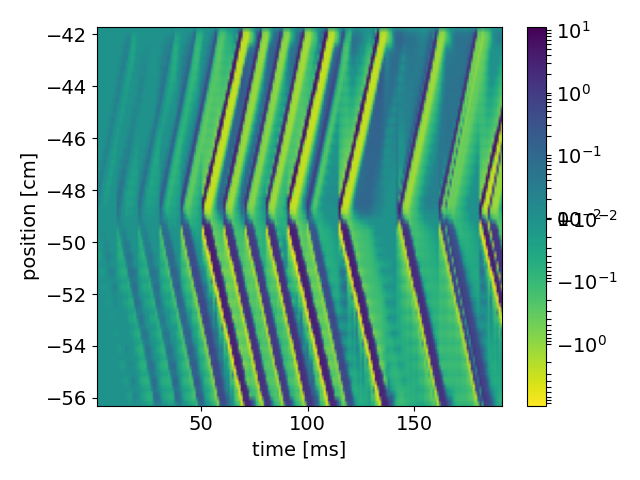
\includegraphics[width=\textwidth]{images/results/application/2_multidomain.png}%
%    \caption{Multidomain}%
%    \label{fig:2_multidomain}%
%  \end{subfigure}
%  \quad
%  \begin{subfigure}[t]{0.48\textwidth}%
%    \centering%
%    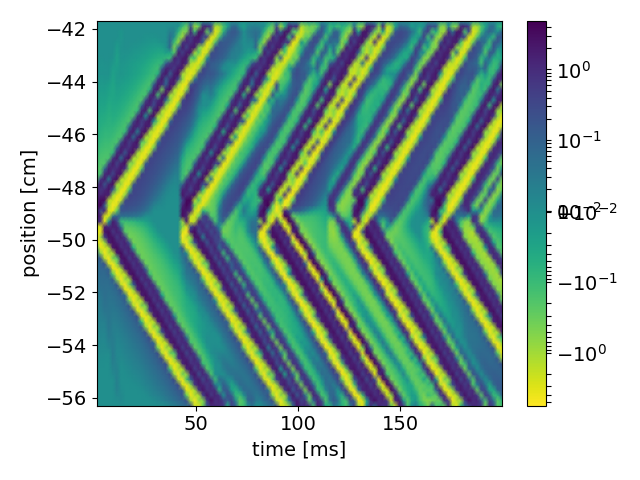
\includegraphics[width=\textwidth]{images/results/application/2_fibers.png}%
%    \caption{Fibers}%
%    \label{fig:2_fibers}%
%  \end{subfigure}   
%  \caption{Fibers and Multidomain}%
%  \label{fig:multidomain_fibers}%
%\end{figure}%


\begin{reproduce_no_break}
  The two simulations in this section with 4 and 25 MUs, respectively, which are visualized in \cref{fig:multidomain_4mus,fig:multidomain_4mus_2,fig:multidomain_25mus2}, can be executed by the following commands:
  \begin{lstlisting}[columns=fullflexible,breaklines=true,postbreak=\mbox{\textcolor{gray}{$\hookrightarrow$}\space}]
    cd $\$$OPENDIHU_HOME/examples/electrophysiology/multidomain/multidomain_with_fat/build_release
    mpirun -n 128 multidomain_with_fat ../settings_multidomain_with_fat.py 4mus.py --n_subdomains 8 1 16
    mpirun -n 126 ./multidomain_with_fat_emg ../settings_multidomain_with_fat.py all_active.py --n_subdomains 6 1 21
  \end{lstlisting}
  For other available numbers of processes, the subdomains at the end of the commands have to be adjusted.
\end{reproduce_no_break}

% ----------------
%
% =================

%-----
% ==================
%
% =-------------------
%-----

\section{Simulation of Coupled Electrophysiology and Solid Mechanics}\label{sec:coupled_electrophysiology_and_solid_mechanics}

Simulating muscle contraction with a detailed model, which accurately describes motor recruitment,
yields the basis for new insights into the neuromuscular orchestration of processes that lead to muscle force generation.

We couple the two model approaches for electrophysiology, the fiber based model presented in \cref{sec:results_fiber_based_electrophysiology} and the multidomain model presented in \cref{sec:solver_multidomain_model}, with a solid mechanics model. 
In \cref{sec:solver_solid_mechanics}, we demonstrated the solver for nonlinear hyperelasticity models in simulations of the passive behavior of muscle tissue. The current section aims at simulating active muscle contraction.

\Cref{sec:fiber_based_contraction} couples the fiber based electrophysiology model with a model of muscle contraction. \Cref{sec:prestress_contraction} discusses an algorithm to add prestress to the description. \Cref{sec:multidomain_contraction} demonstrates the coupling of the multidomain model with the model of muscle contraction. \Cref{sec:volume_coupling_contraction} and \cref{sec:surface_coupling_contraction} describe simulations using the numerical coupling library preCICE.

\subsection{Fiber Based Electrophysiology and Muscle Contraction}\label{sec:fiber_based_contraction}
%-----

We begin with coupling the fiber based electrophysiology solver with the solid mechanics model to simulate muscle contraction as a result of the activation of muscle fibers.
We use the subcellular model of Shorten et al. \cite{Shorten2007}. It computes the microscopic activation parameter $\gamma \in [0,1]$, which is related to the concentration of attached cross-bridges in the sarcomeres. The parameter $\gamma$ is mapped and homogenized from the 0D subcellular points to $\bar{\gamma}$ on the 3D mesh. In the macroscopic 3D mechanics description, the factor is multiplied with a maximum active stress parameter $S_\text{max,active}$ and a force-velocity characteristic $f_l(\lambda_f)$, as described in \cref{sec:material_nonlinear_model}.
The 3D mechanics model updates the geometry of the 3D domain and transfers the fiber stretch value $\lambda_f$ and the contraction velocity $\dot{\lambda}_f$ back to the subcellular model.

In this scenario, we aim to simulate a rapid and strong contraction of the biceps muscle.
The scenario contains 169 fibers, which are associated with 15 MUs. This association is generated by method 1 in \cref{sec:method1_assignment}. All MUs are subsequently activated in a ramp in the first $\SI{1.4}{\s}$. 

The muscle geometry is fixed at its lower end and no external forces are considered in this scenario. The dynamic formulation with the transversely isotropic Mooney-Rivlin material is used, as described in \cref{sec:material_nonlinear_model}.
The 3D muscle mesh contains $2 \times 3 \times 18 = 108$ elements with quadratic finite element ansatz functions and 1295 nodes in total and is  partitioned into subdomains for four processes. Time step widths of $\dt_\text{0D} = \dt_\text{1D} = \dt_\text{splitting} = \SI{1e-4}{\ms}$ and $\dt_\text{3D}=\SI{1}{\ms}$ are used. The used numerical solvers and other settings of the electrophysiology and contraction models are equal to the described scenarios in \cref{sec:simfiber_mu,sec:effects_of_the_mesh_width_emg} and \cref{sec:comparison_linear_nonlinear}.

% normal muscle contraction
%0/4 : This is opendihu 1.2, built Apr 16 2021, C++ 201402, GCC 10.2.0, current time: 2021/4/17 19:56:16, hostname: ipvs-epyc1, n ranks: 4
%0/4 : Open MPI v3.1.6, package: Open MPI maierbn@ipvs-epyc1 Distribution, ident: 3.1.6, repo rev: v3.1.6, Mar 18, 2020
%0/4 : File "../settings_biceps_contraction.py" loaded.
%0/4 : ---------------------------------------- begin python output ----------------------------------------
%Loading variables from "15mus.py".
%scenario_name: 15mus,  n_subdomains: 2 1 2,  n_ranks: 4,  end_time: 4000.0
%dt_0D:           1e-04, diffusion_solver_type:      cg
%dt_1D:           1e-04, potential_flow_solver_type: gmres
%dt_splitting:    1e-04, emg_solver_type:            cg, emg_initial_guess_nonzero: False
%dt_3D:           1e+00, paraview_output: True
%output_timestep: 1e+00  stimulation_frequency: 0.1 1/ms = 100.0 Hz
%fast_monodomain_solver_optimizations: True, use_analytic_jacobian: True, use_vc: True
%fiber_file:              ../../../../input/left_biceps_brachii_13x13fibers.bin
%fat_mesh_file:           ../../../../input/left_biceps_brachii_13x13fibers.bin_fat.bin
%cellml_file:             ../../../../input/new_slow_TK_2014_12_08.c
%fiber_distribution_file: ../../../../input/MU_fibre_distribution_15MUs_13x13fibers.txt
%firing_times_file:       ../../../../input/MU_firing_times_always.txt
%********************************************************************************
%prefactor: sigma_eff/(Am*Cm) = 0.0132 = 3.828 / (500.0*0.58)
%diffusion solver type: cg
%n fibers:              169 (13 x 13), sampled by stride 2 x 2
%n points per fiber:    1481, sampled by stride 40
%4 ranks, partitioning: x2 x y1 x z2
%13 x 13 = 169 fibers, per partition: 6 x 12 = 72
%per fiber: 1D mesh    nodes global: 1481, local: 760
  %sampling 3D mesh with stride 2 x 2 x 40 
 %quadratic 3D mesh    nodes global: 5 x 7 x 37 = 1295, local: 2 x 7 x 18 = 252
 %quadratic 3D mesh elements global: 2 x 3 x 18 = 108, local: 1 x 3 x 9 = 27
%number of degrees of freedom:
                    %1D fiber:       1481  (per process: 760)
            %0D-1D monodomain:      82936  (per process: 42560)
 %all fibers 0D-1D monodomain:   14016184  (per process: 3064320)
                 %3D bidomain:       1295  (per process: 252)
                       %total:   14017479  (per process: 3064572)

% contraction fibers
\begin{figure}
  \centering%
  \begin{subfigure}[t]{0.3\textwidth}%
    \centering%
    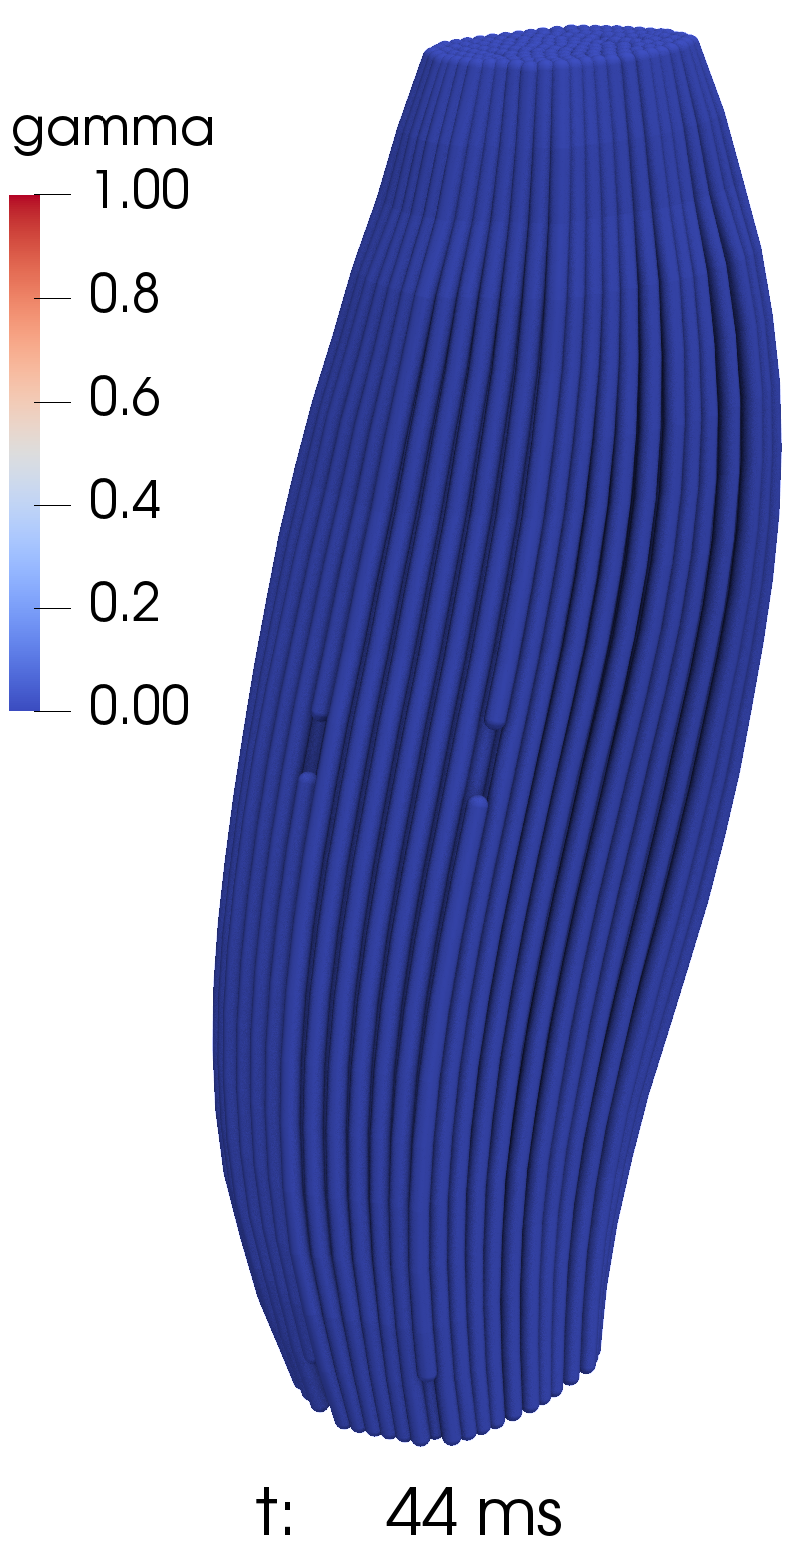
\includegraphics[height=9cm]{images/results/application/contraction_fibers_044.png}%
    \caption{}%
    \label{fig:contraction_fibers_044}%
  \end{subfigure} \,
  \begin{subfigure}[t]{0.18\textwidth}%
    \centering%
    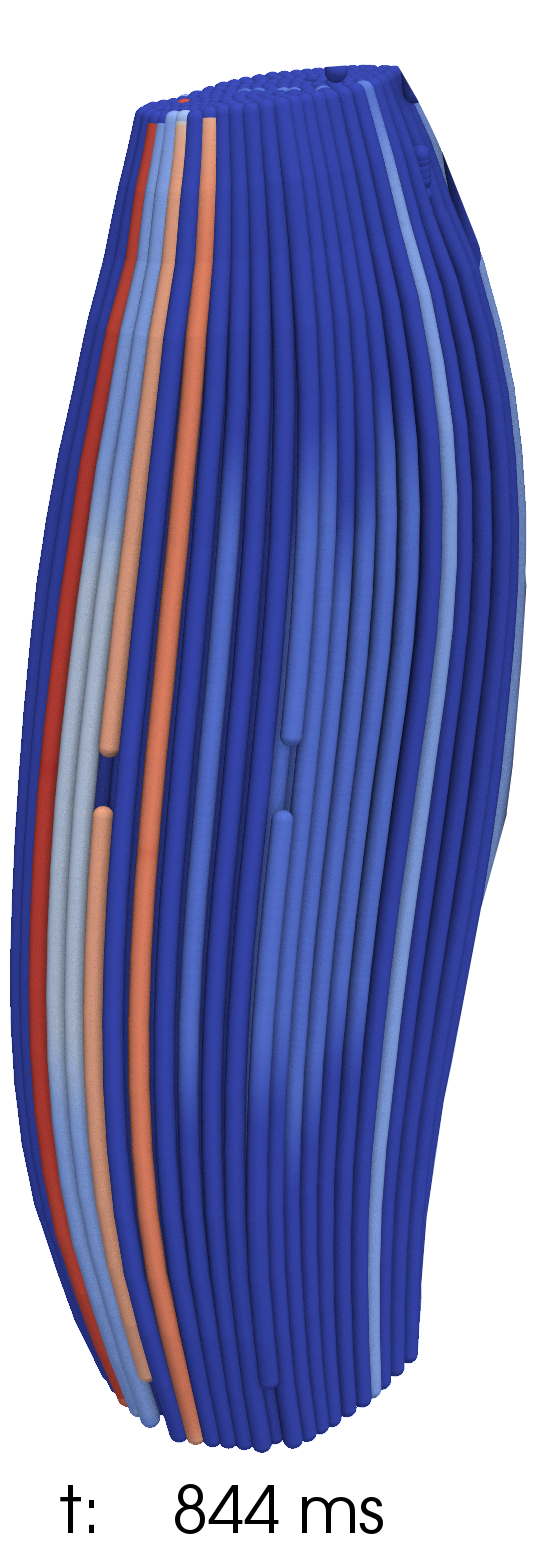
\includegraphics[height=9cm]{images/results/application/contraction_fibers_844b.png}%
    \caption{}%
    \label{fig:contraction_fibers_844b}%
  \end{subfigure}\,
  \begin{subfigure}[t]{0.25\textwidth}%
    \centering%
    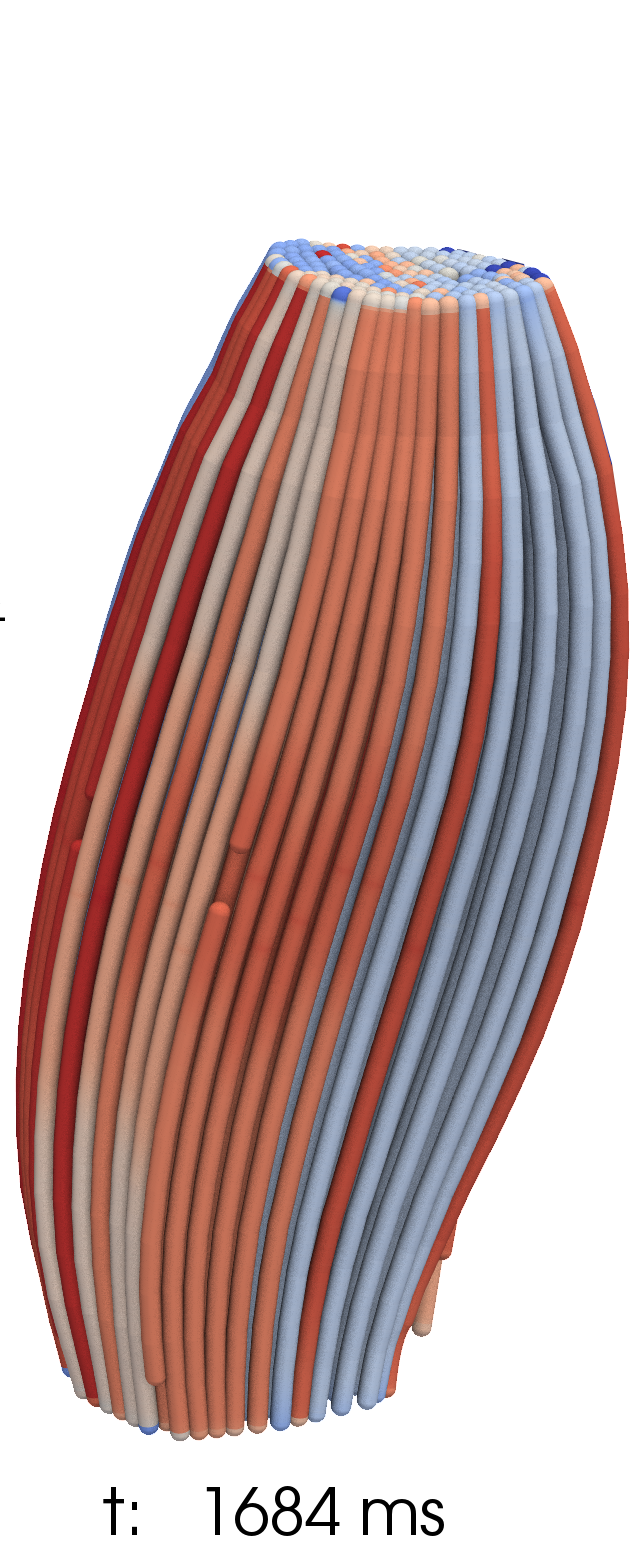
\includegraphics[height=9cm]{images/results/application/contraction_fibers_1684b.png}%
    \caption{}%
    \label{fig:contraction_fibers_1684b}%
  \end{subfigure}\,
  \begin{subfigure}[t]{0.2\textwidth}%
    \centering%
    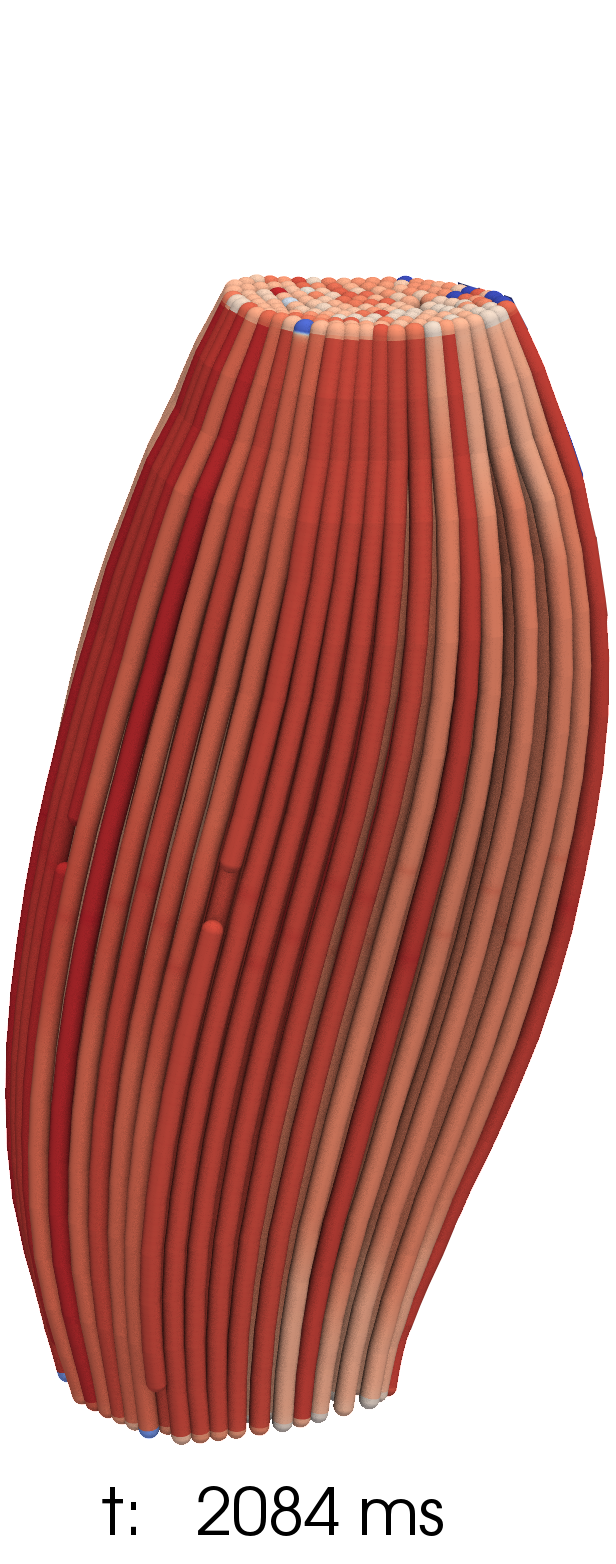
\includegraphics[height=9cm]{images/results/application/contraction_fibers_2084b.png}%
    \caption{}%
    \label{fig:contraction_fibers_2084b}%
  \end{subfigure}
  \caption{Simulation of fiber based electrophysiology and muscle contraction: Activation of the muscle fibers and overall deformation at various timesteps.}%
  \label{fig:contraction_fibers_1}%
\end{figure}%

\Cref{fig:contraction_fibers_1} shows the fibers of the contracting muscle at four different timesteps between $t=\SI{44}{\ms}$ and $t=\SI{2.084}{\s}$. The fibers are colored according to the resulting activation parameter $\gamma$, which is a measure for the generated force on the sarcomere level. Between $t=\SI{44}{\ms}$ and $t=\SI{844}{\ms}$, shown in \cref{fig:contraction_fibers_044,fig:contraction_fibers_844b}, the smallest MUs are activated, which, in this example, are mainly located on the left-hand side. As a consequence, the muscle domain initially bends slightly to the left. As more MUs become active at $t=\SI{1684}{\ms}$, depicted in \cref{fig:contraction_fibers_1684b}, the deformation increases and the bending direction is reversed. However, the fibers on the left-hand side still exhibit the highest $\gamma$ value, as they have been stimulated most often at that time.
At $t=\SI{1684}{\ms}$, visualized in \cref{fig:contraction_fibers_2084b}, almost all fibers have a $\gamma$ value close to one, corresponding to full activation.

% contracted state
\begin{figure}
  \centering%
  \begin{subfigure}[t]{0.31\textwidth}%
    \centering%
    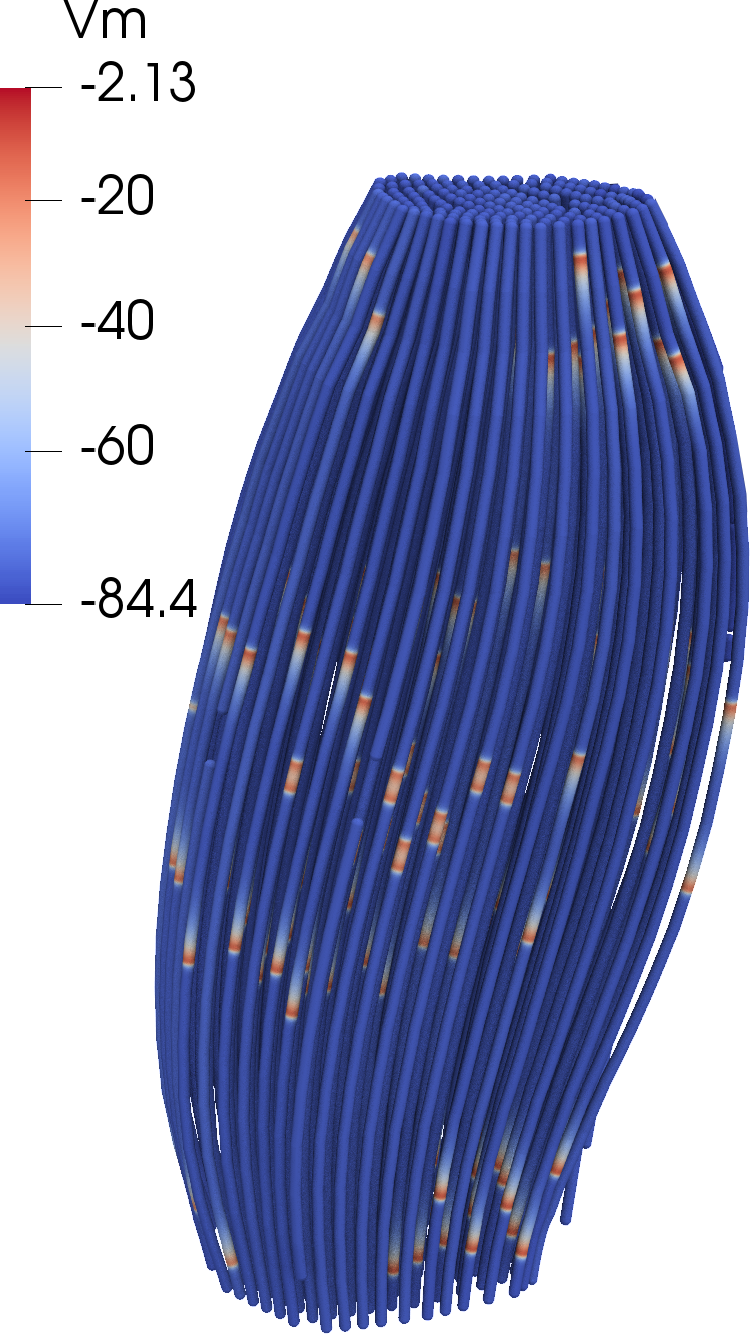
\includegraphics[height=77mm]{images/results/application/contraction_fibers.png}%
    \caption{Action potentials given by the membrane voltage $V_m$ (in millivolts) on the muscle fibers.}%
    \label{fig:contraction_fibers}%
  \end{subfigure}\,
  \begin{subfigure}[t]{0.31\textwidth}%
    \centering%
    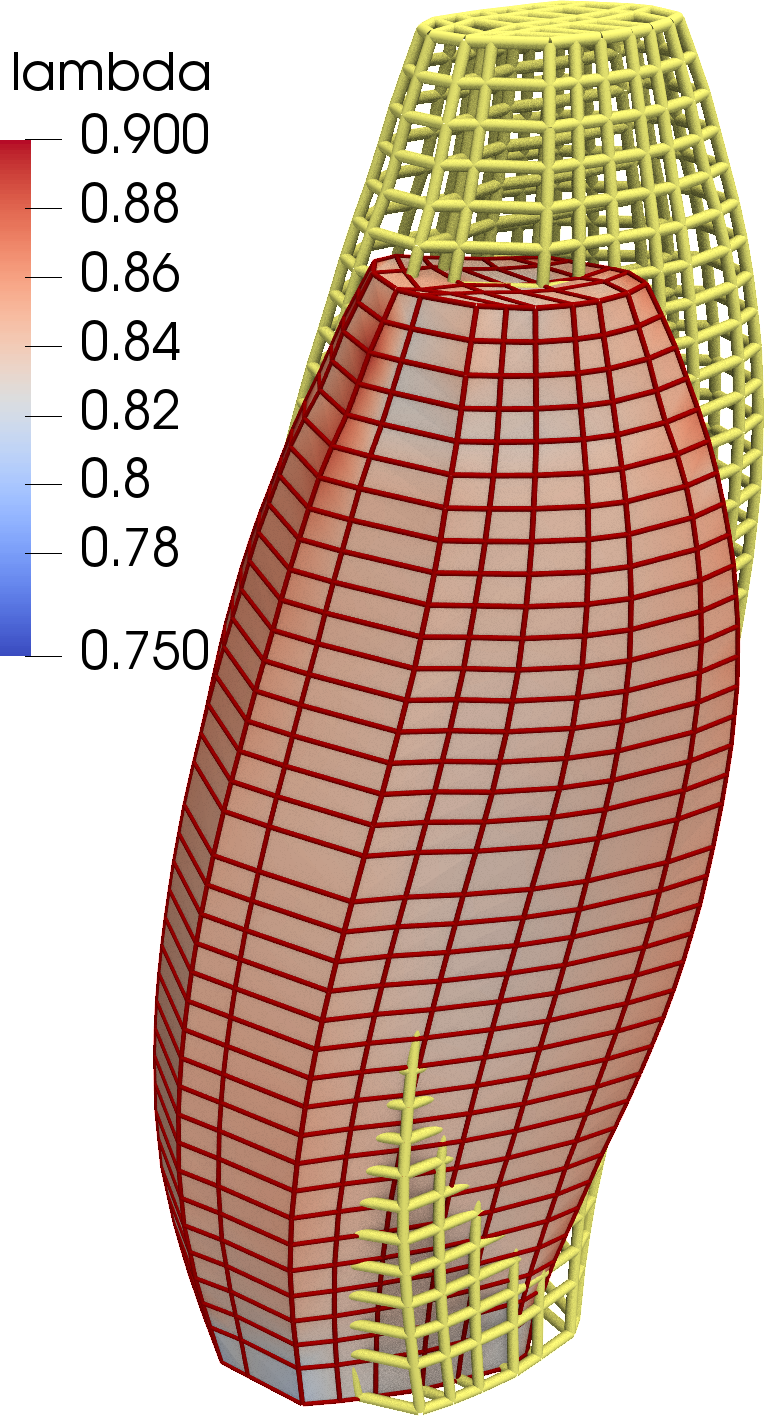
\includegraphics[height=8cm]{images/results/application/contraction_lambda.png}%
    \caption{Stretch parameter $\lambda$ of the deformed 3D muscle domain (red mesh) in comparison to the reference configuration (yellow mesh).}%
    \label{fig:contraction_lambda}%
  \end{subfigure}
  \begin{subfigure}[t]{0.31\textwidth}%
    \centering%
    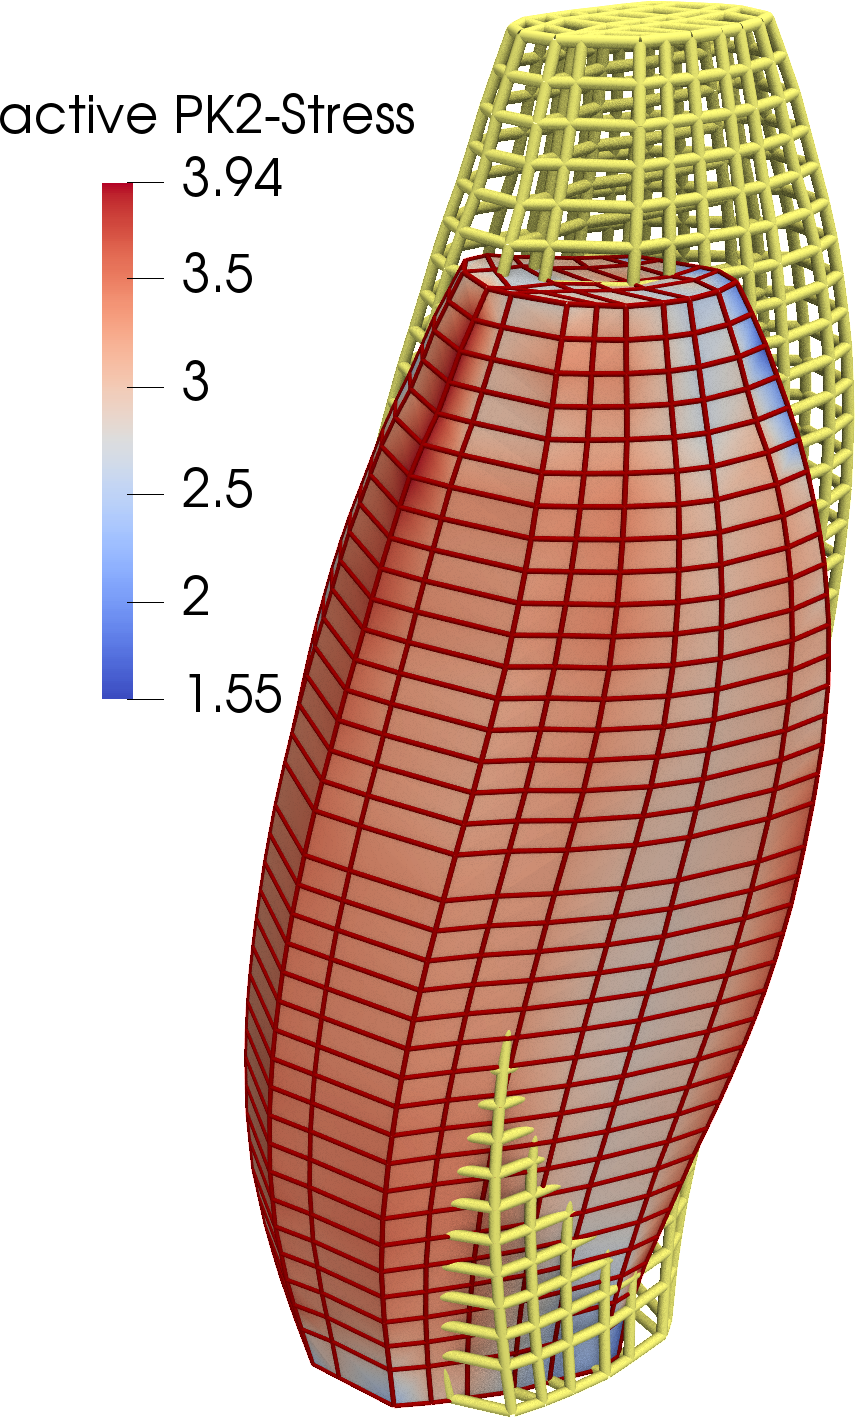
\includegraphics[height=8cm]{images/results/application/contraction_active_stress.png}%
    \caption{Value of the active second Piola-Kirchhoff stress.}%
    \label{fig:contraction_active_stress}%
  \end{subfigure}
  \caption{Simulation of fiber based electrophysiology and muscle contraction: Simulation results at $t=\SI{2084}{\ms}$.}%
  \label{fig:contraction_at_end}%
\end{figure}%

\Cref{fig:contraction_at_end} shows several variables at the simulation end time of $t=\SI{2084}{\ms}$. \Cref{fig:contraction_fibers} visualizes the transmembrane voltage $V_m$ on the muscle fibers. Action potentials can be seen on almost all fibers, as the whole muscle is activated at this time. \Cref{fig:contraction_lambda} shows a comparison between the reference configuration given by the yellow mesh and the current configuration given by the red mesh. The muscle domain is colored according to the stretch $\lambda$, which has a nearly constant value of $\lambda \approx \SI{85}{\percent}$ at the end time of this scenario. A similar visualization is given in \cref{fig:contraction_active_stress} for the active stress in the muscle.

Because of the high level of activation and the corresponding active stress distribution in the muscle, our mechanics solver only converges up to the shown simulation time of \SI{2084}{\ms} in this scenario. The aim of the scenario is to simulate the contraction of a fully activated muscle. Other scenarios, where the activation is applied more slowly, allow for a convergence of the mechanics solver during longer simulation time spans.

The presented scenario showed that a fully activated biceps muscle contracted to about \SI{85}{\percent} of its original length. However, in reality, larger contractions are possible. In the shown scenario, the muscle was initially in a stress-free configuration. More realistic scenarios can incorporate pretension forces, where the undeformed reference configuration is subject to a constant stress level in the muscle's direction of the line of action. This is considered in the next scenario.

% muscle contraction
%\begin{figure}
%  \centering%
%  \includegraphics[width=0.5\textwidth]{images/results/application/neuromuscular_muscle_contraction_traction.png}%
 % \caption{contraction traction}%
%  \label{fig:neuromuscular_muscle_contraction_traction}%
%\end{figure}%

\begin{reproduce}
  The simulation in this section can be run as follows:
  \begin{lstlisting}[columns=fullflexible,breaklines=true,postbreak=\mbox{\textcolor{gray}{$\hookrightarrow$}\space}]
    cd $\$$OPENDIHU_HOME/examples/electrophysiology/fibers/fibers_contraction/no_precice/build_release
    mpirun -n 4 ./biceps_contraction ../settings_biceps_contraction.py ramp.py
  \end{lstlisting}
\end{reproduce}

\subsection{Simulation of Prestress}\label{sec:prestress_contraction}
% compressing muscle by external force does not work -> need activation 

To obtain more realistic ranges of muscle contraction, a nonzero, constant prestress can be considered in the undeformed configuration of the muscle. 
In our solid mechanics formulation, the reference configuration always has zero stress. Thus, we need to construct a separate, first reference configuration of a shorter muscle geometry. We stretch it to the original muscle length by applying external forces. The resulting, second configuration resembles the original muscle geometry and has the desired prestress characteristics.

The detailed steps of this algorithm are visualized in \cref{fig:neuromuscular_prestretch} and are described in the following.
We begin with the given geometry of the muscle with body fat layer, which is shown as black wireframe mesh in \cref{fig:neuromuscular_prestretch_1}. In a first static simulation step, a constant active stress $\alpha_\text{pre}\,S_\text{max,active}$ is prescribed in the entire muscle volume. The resulting muscle deformation is computed, using the usual nonlinear hyperelastic muscle material. $S_\text{max,active}$ refers to the maximum active stress value as used in the mechanics model description in \cref{eq:active_stress_term}. The result of this first step is a shortened muscle with the same volume as the original geometry. \Cref{fig:neuromuscular_prestretch} shows the result by the yellow volume for $\alpha_\text{pre}=0.3$. It can be seen that the length of the muscle has shortened by approximately \SI{13}{\percent}.

In the second step, we reuse the computed deformed geometry of the first step as new stress-free reference configuration and re-extend it by applying a constant surface load $F_\text{pre}$ pointing to the bottom on the lower face in the setting of \cref{fig:neuromuscular_prestretch}. The value of $F_\text{pre}$ corresponding to $\alpha_\text{pre}$ has to be estimated by numerical experiments.

This step is again solved as a static problem. The result is a similar muscle geometry as the original one, and contains prestress according to the applied force. The muscle volume is exactly preserved due to the incompressible material formulation. \Cref{fig:neuromuscular_prestretch_2} shows the starting point for the second step by the black wireframe mesh and the resulting geometry for a total applied force of $F_\text{pre}=\SI{30}{\newton}$ by the red volume. The comparison of the original, black mesh in \cref{fig:neuromuscular_prestretch_1} with the red volume in \cref{fig:neuromuscular_prestretch_2} shows a good match of the geometry.
For the subsequent dynamic simulations of, e.g., muscle contraction, the surface load has to be constantly applied. It corresponds to the tendon forces and the loads of the musculoskeletal system acting on the muscle.

The active stress parameter $\alpha_\text{pre}$ and the corresponding preload force $F_\text{pre}$ can be chosen according to the desired amount of prestress. However, the higher these values are chosen, the more difficult is it for the nonlinear solid mechanics solvers to converge to a solution. Especially for irregular or large mechanics meshes, a lower stress factor of, e.g., $\alpha_\text{pre}=0.1$ has to be chosen. To improve convergence, we apply the load in the second step of the algorithm incrementally by several load steps. In addition, reducing the number of unknowns and increasing the mesh width in the mechanics problem can help, as this improves the conditioning of the problem. 
 
% contracted state
\begin{figure}
  \centering%
  \hfill
  \begin{subfigure}[t]{0.48\textwidth}%
    \centering%
    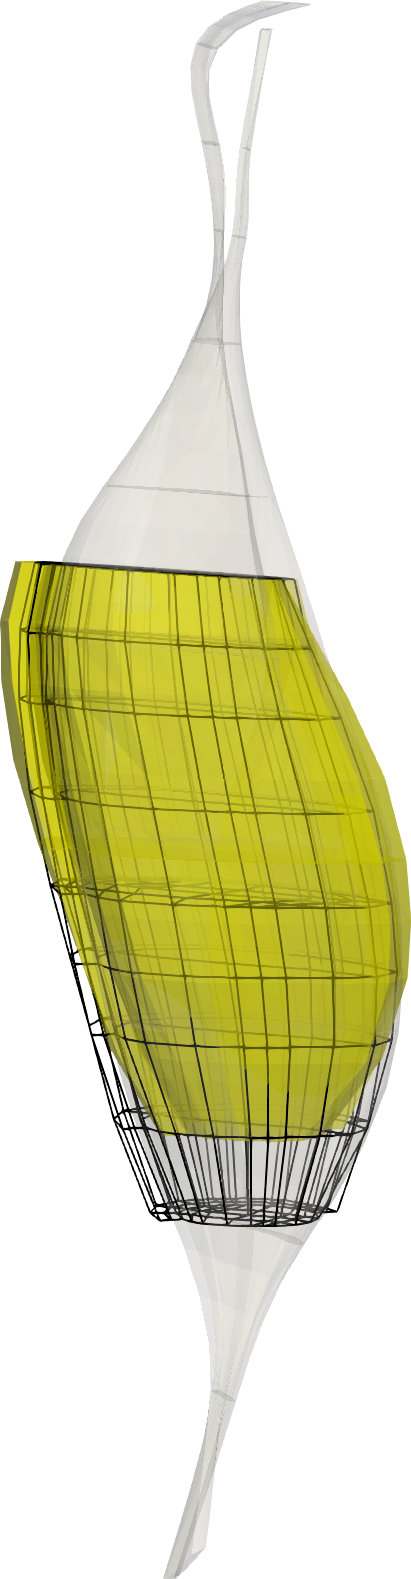
\includegraphics[height=12cm]{images/results/application/neuromuscular_prestretch_1.png}%
    \caption{In the first step, the original mesh (black wireframe) is contracted by an artificial active stress $\alpha_\text{pre}\,S_\text{max,active}$ to yield a shortened muscle (yellow mesh).}%
    \label{fig:neuromuscular_prestretch_1}%
  \end{subfigure}\hfill
  \begin{subfigure}[t]{0.48\textwidth}%
    \centering%
    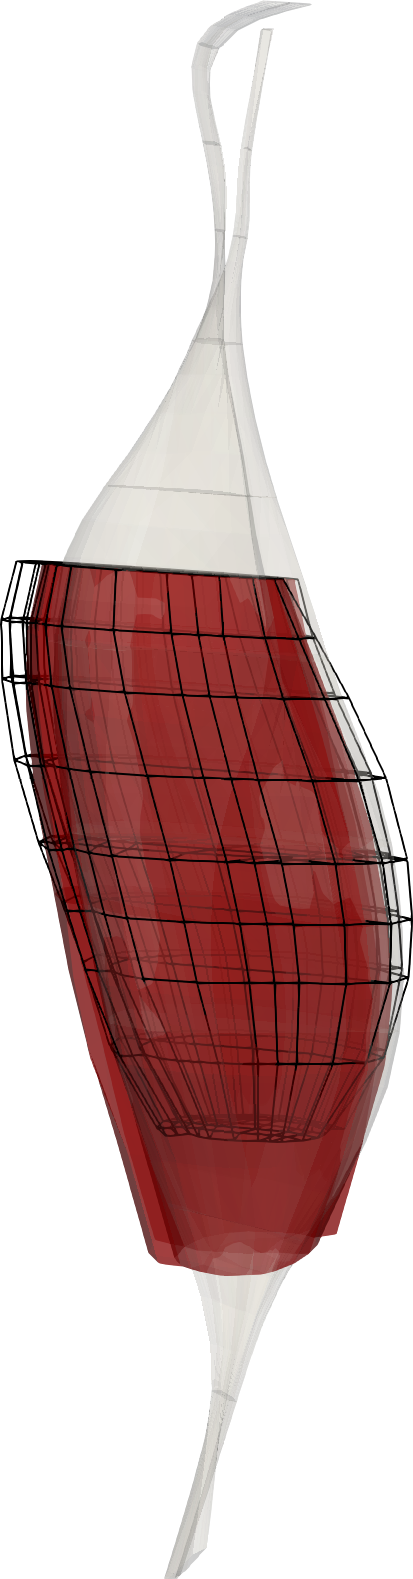
\includegraphics[height=12cm]{images/results/application/neuromuscular_prestretch_2.png}%
    \caption{In the second step, the mesh is extended again by an external surface load. The black wireframe corresponds to the yellow volume in (a), the red volume is the resulting geometry.}%
    \label{fig:neuromuscular_prestretch_2}%
  \end{subfigure}
  \hfill
  \caption{Simulation of biceps muscle geometry with prestress: The two steps of the algorithm to generate a reference geometry with prestress, shown with the geometry of the tendons for reference.}%
  \label{fig:neuromuscular_prestretch}%
\end{figure}%


\subsection{Coupling of the Multidomain Model and Solid Mechanics Model with Prestress}\label{sec:multidomain_contraction}

In the following, we present a scenario that uses the prestress algorithm of the last section and couples the multidomain and mechanics models to simulate surface EMG signals on the skin surface over a contracting muscle.

We choose $\alpha_\text{pre}=0.1$ and apply the prestretch force $F_\text{pre}=\SI{10}{\newton}$ in three load steps. The multidomain model considers 5 MUs with stimulation frequencies between \SI{7}{\hertz} and \SI{24}{\hertz} and a 3D mesh of $8 \times 8 \times 28 = 1792$ elements. We execute the simulation with four processes. All other parameters and settings of the multidomain model and the solid mechanics model that are not explicitly mentioned in the following are chosen the same as in \cref{sec:multidomain_components} and \cref{sec:comparison_linear_nonlinear}.

For the discretization of the mechanics model, we use a coarser mesh than for the multidomain model. Furthermore, we use quadratic elements instead of linear elements. The Python implementation of the settings script of this example contains functionality to create the mechanics mesh by subsampling the multidomain mesh with specified factors. In the current scenario, we set these factors for the $x$, $y$ and $z$ directions to 0.7, 0.7, and 0.3, respectively. As a result, we get meshes with $5 \times 7 \times 9 = 315$ elements for the muscle and $5 \times 1 \times 4 = 20$  elements for the body fat domain. \Cref{fig:multidomain_prestretch5} visualizes all meshes used in this scenario: The orange muscle mesh and the red body mesh are used for the multidomain model, and the yellow mesh is used for the solid mechanics model.


% multidomain prestretch
\begin{figure}
  \centering%
  \hfill
  \begin{subfigure}[t]{0.31\textwidth}%
    \centering%
    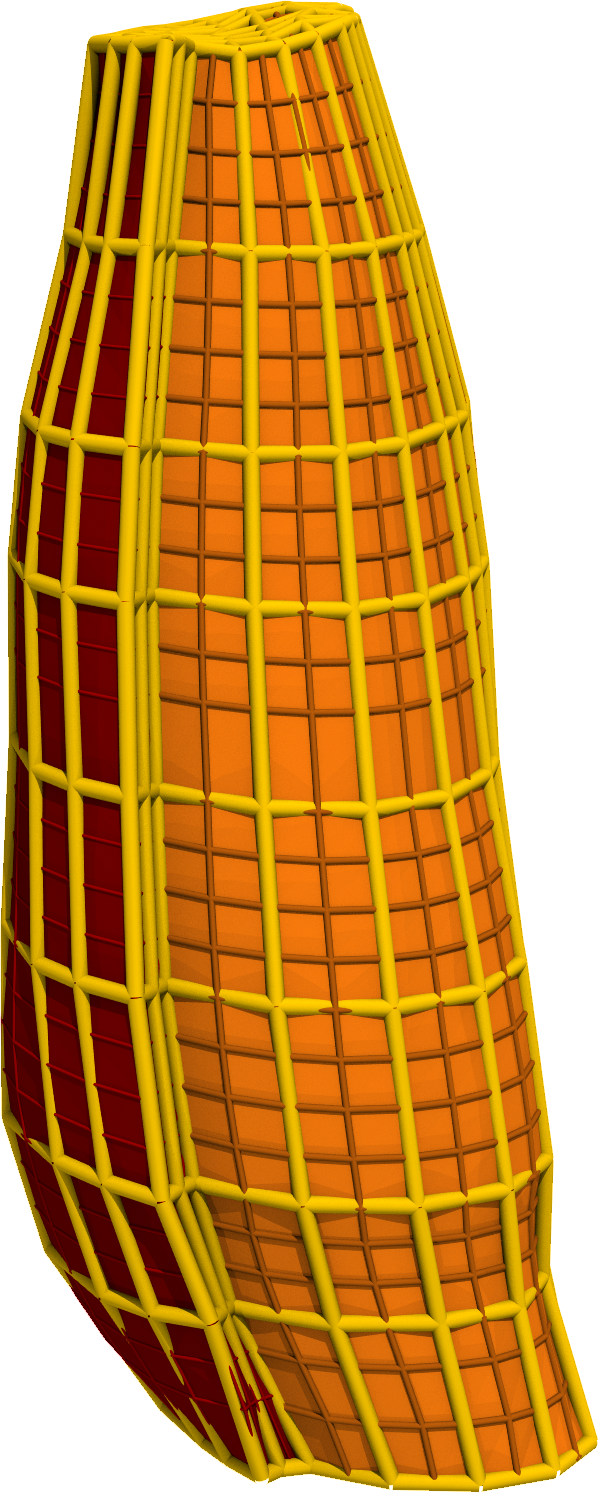
\includegraphics[height=87mm]{images/results/application/multidomain_prestretch5.png}%
    \caption{Multidomain meshes of the muscle domain (orange), body fat domain (red) and the coarser mesh used for the solid mechanics model (yellow).}%
    \label{fig:multidomain_prestretch5}%
  \end{subfigure}
  \begin{subfigure}[t]{0.31\textwidth}%
    \centering%
    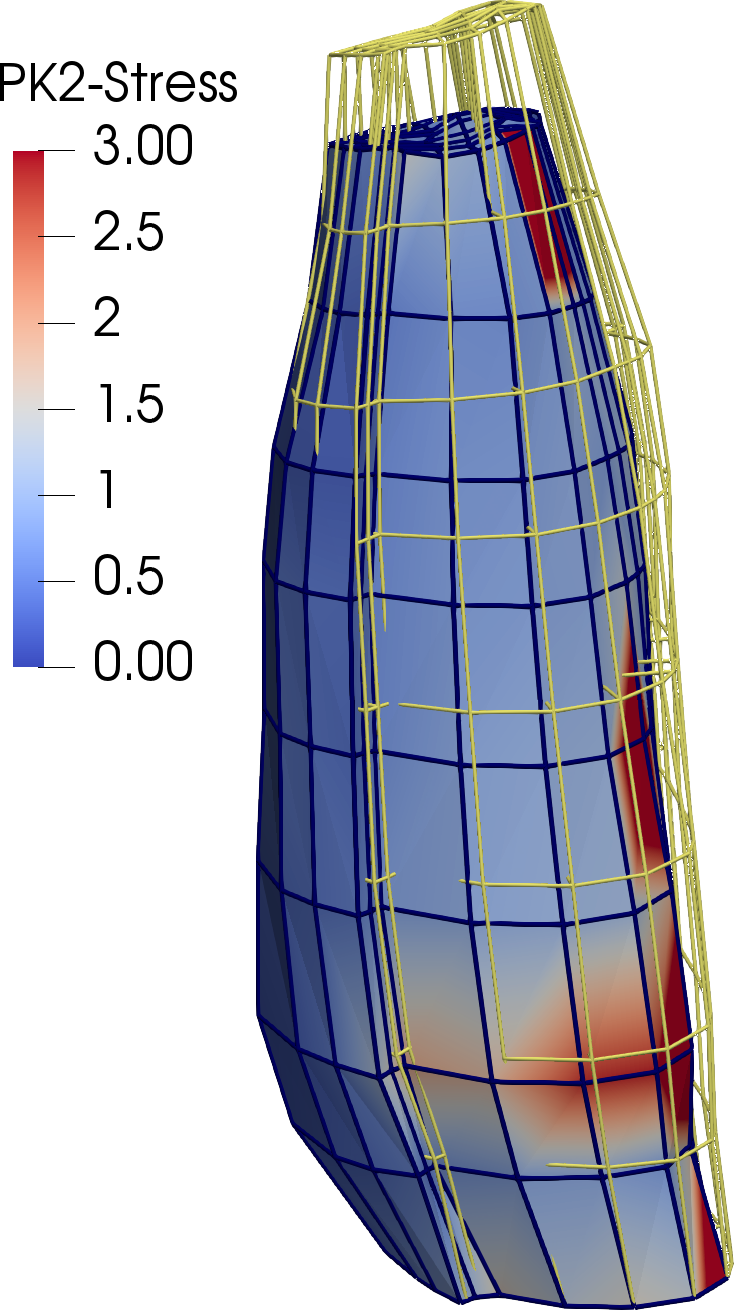
\includegraphics[height=95mm]{images/results/application/multidomain_prestretch6.png}%
    \caption{Reference configuration (yellow mesh) and current configuration of the muscle colored according to the distribution of the second Piola-Kirchhoff stress.}%
    \label{fig:multidomain_prestretch6}%
  \end{subfigure}\qquad
  \begin{subfigure}[t]{0.31\textwidth}%
    \centering%
    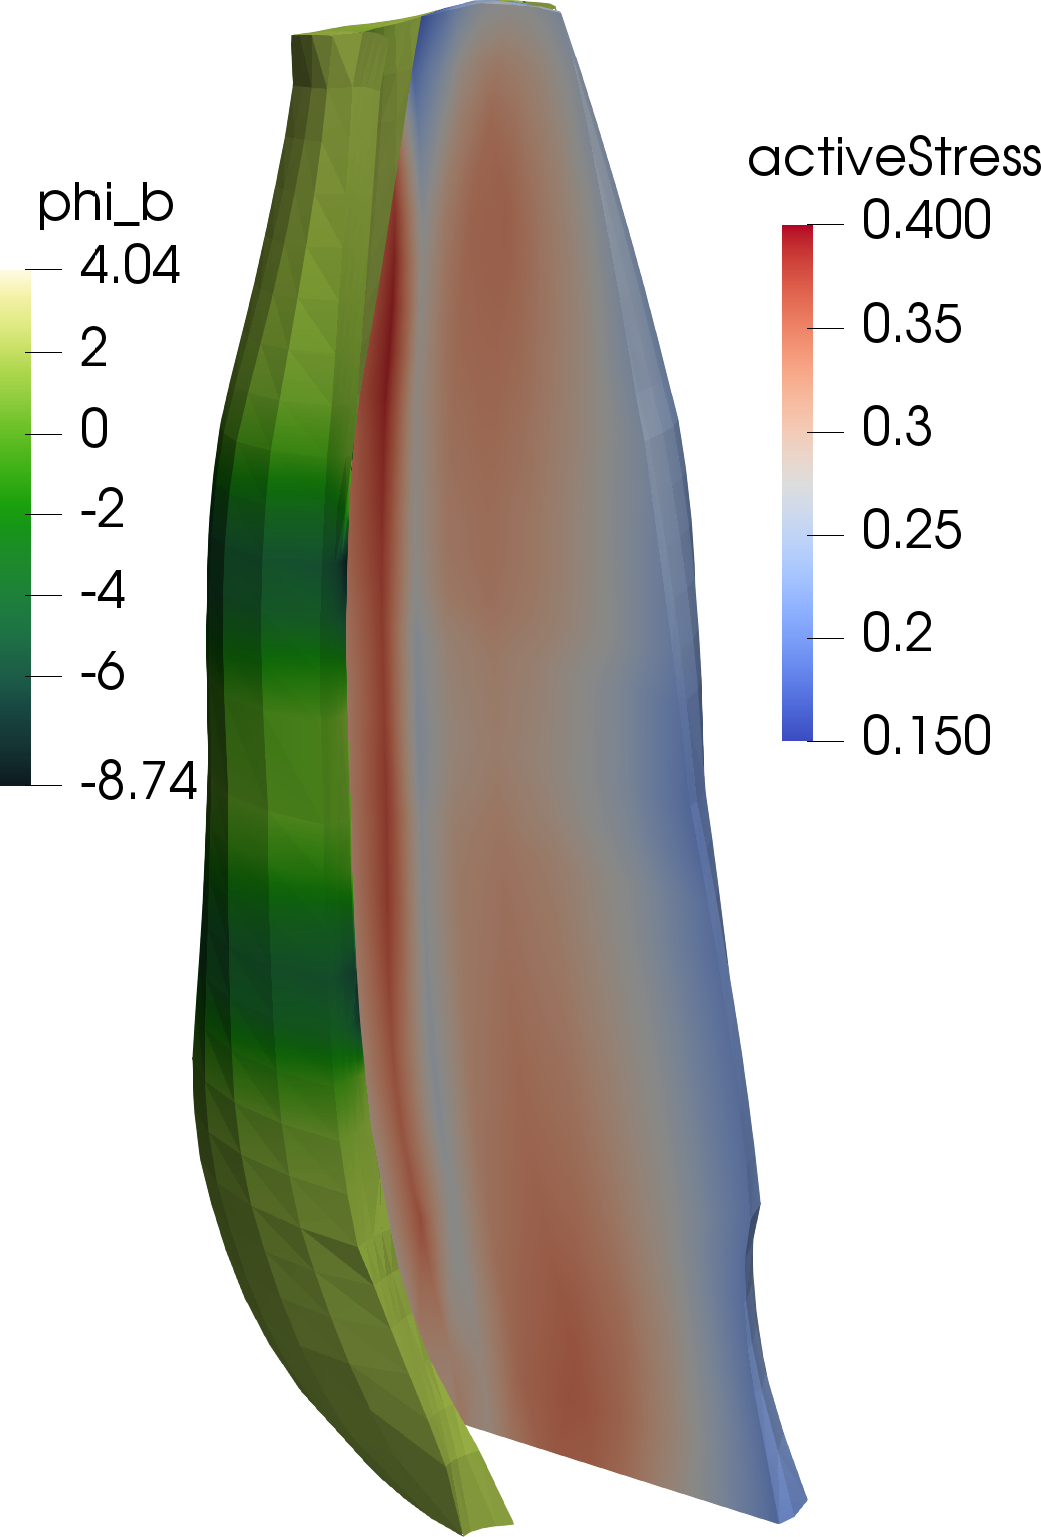
\includegraphics[height=87mm]{images/results/application/multidomain_prestretch2.png}%
    \caption{Electric potential $\phi_b$ in the body domain (green color scale, in millivolts) and active stress in the interior of the muscle (blue-red color scale, in \SI{}{\newton\per\centi\meter\squared}).}%
    \label{fig:multidomain_prestretch2}%
  \end{subfigure}
  \hfill
  \caption{Simulation of muscle contraction based on the multidomain model with prestressed muscle geometry: Used meshes and simulation results at $t=\SI{920}{\ms}$ of a scenario of the multidomain electrophysiology model coupled to the solid mechanics model.}%
  \label{fig:multidomain_prestretch}%
\end{figure}%

\Cref{fig:multidomain_prestretch6,fig:multidomain_prestretch2} depict results of the simulation at time $t=\SI{920}{\milli\second}$. 
\Cref{fig:multidomain_prestretch6} shows the reference geometry by the yellow wireframe after applying the prestress. The muscle is colored according to the value of the second Piola-Kirchhoff stress. During this dynamic simulation, the muscle bends elastically slightly to the left and right, as it is only fixed at its bottom in \cref{fig:multidomain_prestretch}. This explains the stress distribution at the snapshot for $t=\SI{920}{\milli\second}$ in \cref{fig:multidomain_prestretch6}, where higher stresses occur on the right-hand side.

\Cref{fig:multidomain_prestretch2} shows the electric potential $\phi_b$ of the body domain by the green color scale on the left of the image. The visible part of the fat layer shows two action potentials, visualized by the two dark green stripes.

Moreover, \cref{fig:multidomain_prestretch2} displays the total active stress  $\bfS_\text{active}$ in the interior of the muscle by the color scale that ranges from blue to red color. In the multidomain model, $\bfS_\text{active}$ is calculated as a weighted sum over the contributions $\bfS_\text{active}^k$ of the MU compartments, scaled by the occupancy factors $f_r^k$ (cf. \cref{sec:multidomain_model}):
\begin{align*}
  \bfS_\text{active} = \sum\limits_{k=1}^{N_\text{MU}} f_r^k\,\bfS_\text{active}^k.
\end{align*}
The muscle domain in \cref{fig:multidomain_prestretch2} is cut open, such that interior distribution at the cut plane can be seen. The image shows two regions of higher active stress, which run vertically through the muscle, given by red color. They are a result on the location of the MUs in this scenario. The legend shows that the active stress inside the muscle is below $\SI{0.4}{\newton\per\centi\meter\squared}$, while the maximum active stress parameter is chosen as $S_\text{max,active}=\SI{7.3}{\newton\per\centi\meter\squared}$. This low activation level is a result of the chosen MU recruitment. As a result, the muscle only slightly contracts, as can be seen in \cref{fig:multidomain_prestretch6}.

In summary, both the fiber based electrophysiology model and the multidomain model can be coupled with the nonlinear solid mechanics model to simulate muscle contraction, as presented in \cref{sec:fiber_based_contraction} and in this section. 
The computational efficiency considerations discussed in the comparison of the fiber based and multidomain approaches in \cref{sec:multidomain_differences} also apply to coupled simulations with muscle contraction. For longer simulation times, the fiber based approach in \cref{sec:fiber_based_contraction} is, therefore, favored.

%0/4 : This is opendihu 1.2, built Apr 17 2021, C++ 201402, GCC 10.2.0, current time: 2021/4/18 17:13:03, hostname: ipvs-epyc1, n ranks: 4            
%0/4 : Open MPI v3.1.6, package: Open MPI maierbn@ipvs-epyc1 Distribution, ident: 3.1.6, repo rev: v3.1.6, Mar 18, 2020
%0/4 : File "../settings_multidomain_prestretch.py" loaded.                                     
%0/4 : ---------------------------------------- begin python output ----------------------------------------                                                                                   
%Loading variables from "multidomain.py".                                                                                                                                                      
%scenario_name: multidomain,  n_subdomains: 2 1 2,  n_ranks: 4,  end_time: 4000.0                                                                                                              
%dt_0D:           1e-03    multidomain solver:         gmres, lumped mass matrix: False                                                                                                        
%dt_multidomain:  1e-03    multidomain preconditioner: euclid, symmetric precond.: True
%dt_splitting:    1e-03    theta: 1.0, solver tolerances, abs: 1e-15, rel: 1e-15
%dt_elasticity:   1e+00    elasticity solver: lu, preconditioner: none
%fiber_file:              /data/scratch/sgs/maierbn/opendihu/examples/electrophysiology/input/left_biceps_brachii_9x9fibers.bin
%fat_mesh_file:           /data/scratch/sgs/maierbn/opendihu/examples/electrophysiology/input/left_biceps_brachii_9x9fibers.bin_fat.bin
%cellml_file:             /data/scratch/sgs/maierbn/opendihu/examples/electrophysiology/input/hodgkin_huxley-razumova.cellml
%firing_times_file:       /data/scratch/sgs/maierbn/opendihu/examples/electrophysiology/input/MU_firing_times_always.txt
%********************************************************************************
%4 ranks, partitioning: x2 x y1 x z2
  %sampling 3D mesh with stride 1 x 1 x 50 
    %linear 3D mesh    nodes global: 9 x 9 x 29 = 2349, local: 4 x 9 x 14 = 504
    %linear 3D mesh elements global: 8 x 8 x 28 = 1792, local: 4 x 8 x 14 = 448
 %quadratic 3D mesh    nodes global: 9 x 9 x 29 = 2349, local: 4 x 9 x 14 = 504
 %quadratic 3D mesh elements global: 4 x 4 x 14 = 224, local: 2 x 4 x 7 = 56
    %fat mesh, n points total:    2465 (17 x 5 x 29), (per process: 4 x 5 x 14 = 280)
   %sub-sampling 3D elasticity mesh with factors 0.7, 0.7, 0.3 
   %elasticity quadratic 3D meshes:
   %muscle:             nodes global: 5 x 7 x 9 = 315, local: 2 x 7 x 4 = 56
          %quadratic elements global: 2 x 3 x 4 = 24, local: 1 x 1 x 2 = 2
   %fat and skin layer: nodes global: 11 x 3 x 9 = 297, local: 2 x 3 x 4 = 24
          %quadratic elements global: 5 x 1 x 4 = 20, local: 1 x 1 x 2 = 2

%Debugging output about compartment firing: Taking input from file "/data/scratch/sgs/maierbn/opendihu/examples/electrophysiology/input/MU_firing_times_always.txt"
%First stimulation times
    %Time  MU compartments
    %0.00   0 [0]
    %0.00   1 [1]
    %0.00   2 [2]
    %0.00   3 [3]
%stimulated MUs: 4, not stimulated MUs: 0
%duration of assembling this list: 0.000 s

%Load relative factors, f_r, from file "compartments_relative_factors.left_biceps_brachii_9x9fibers.bin.5_mus_stride_1x1x50_partitioning_2x1x2"
%MU 0, maximum fr: 0.1999999999999993
%MU 1, maximum fr: 0.4426237526712864
%MU 2, maximum fr: 0.6900999803960008
%MU 3, maximum fr: 0.9425257326752092
%MU 4, maximum fr: 1.1999999999999993



% prestretch
%\begin{figure}
%  \centering%
%  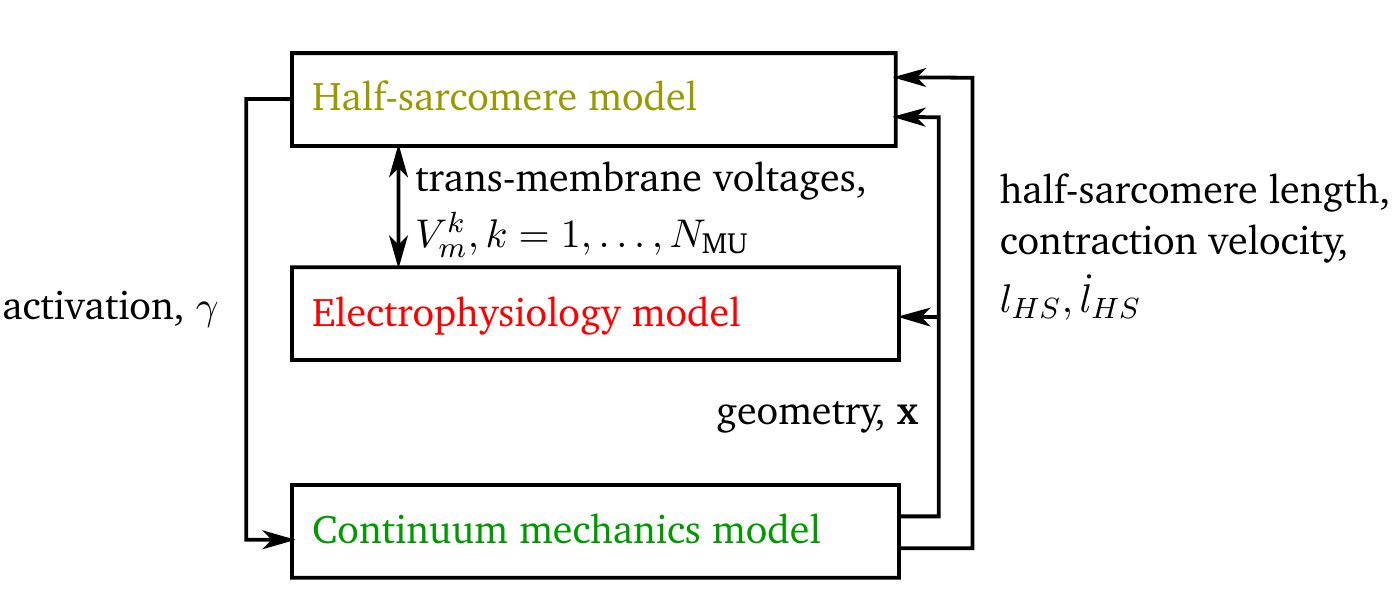
\includegraphics[width=0.5\textwidth]{images/results/application/fibers_muscle_contraction_quantities.png}%
%  \caption{prestretch}%
%  \label{fig:prestrech1b}%
%\end{figure}%

\begin{reproduce_no_break}
  The simulation can be run with the following commands. Instead of four processes also other numbers are possible. A lot of parameters can be fine-tuned in the \code{../variables/multidomain.py} settings file.
  \begin{lstlisting}[columns=fullflexible,breaklines=true,postbreak=\mbox{\textcolor{gray}{$\hookrightarrow$}\space}]
    cd $\$$OPENDIHU_HOME/examples/electrophysiology/multidomain/multidomain_prestretch/build_release
    mpirun -n 4 ./multidomain_prestretch ../settings_multidomain_prestretch.py multidomain.py
  \end{lstlisting}
\end{reproduce_no_break}

% --------
%
% f==============

% ==================
%
% =-------------------
%-----
\subsection{Coupling of Solid Mechanics Models using the Software preCICE}\label{sec:volume_coupling_contraction}

One problem of multi-scale simulations with solid mechanics models is the limited amount of parallelism, 
if a coarse mechanics mesh with a low number of elements is chosen. The domain can only be partitioned into as many subdomains as there are elements in the 3D mechanics mesh. While this is not an issue for small scale simulations like the ones shown in the previous sections, it prohibits exploitation of High Performance Computing resources, e.g., if numerous muscle fibers are considered as in \cref{sec:effects_of_the_mesh_width_emg}.

The reason for the limited parallelism lies in the partitioning scheme, where every node in the 3D domain corresponds to the subdomain of exactly one process, regardless of the mesh. OpenDiHu does not allow to partition, e.g., the finely resolved 1D muscle fiber meshes differently than the coarse 3D mechanics mesh. However, this restriction can be circumvented by using multiple OpenDiHu programs with different partitioning schemes and by performing the data transfer between the meshes using an external coupling software.

We provide support for the black-box coupling library preCICE \cite{precice}. This open source library allows mapping data between different meshes, can communicate values between subdomains that reside on different processors, and implements implicit numerical coupling schemes with quasi-Newton methods. The implementation is known to scale well on small-scale clusters and supercomputers.
The preCICE library targets a minimally-invasive approach, where the user application implements a preCICE adapter. Multiple, potentially different solver codes can be coupled numerically and compute individual model parts of a joint multi-physics simulation. Moreover, preCICE has an active and growing community where experiences and codes are shared, and open source adapters are available for several popular solvers.

This makes the library suited for our use case. We provide two different types of preCICE adapters in OpenDiHu, one for surface coupling of 2D meshes and one for volume coupling of 3D meshes. These adapters integrate with the structure of nested solvers and can be positioned anywhere in the solver tree (cf. \cref{fig:solver_tree_multidomain_spindles}). The meshes and variables that are exposed to preCICE can be configured in the settings file.

In the current section, we show how to use the volume coupling adapter to resolve the initially stated issue of limited scalability for coupled simulations with electrophysiology and mechanics models. Subsequently, the next section presents a simulation that uses surface coupling. Details can also be found in \cite{hlrs2021}.

We simulate muscle contraction and surface EMG of the biceps muscle using the fiber based electrophysiology model. To fully exploit the  capabilities of an 18-core Intel Core i9-10980XE processor, we compute the electrophysiology model using 16 processes and the mechanics model using 2 processes. The data mapping between the differently partitioned 3D meshes is performed by preCICE.

\Cref{fig:precice_muscle_force} shows the structure of the simulation components with the used meshes and the exchanged variables in this simulation. Two different OpenDiHu programs are executed at the same time, given by the gray boxes. The program corresponding to the left box solves the electric conduction problem, given by the bidomain equation \cref{eq:bidomain1} on the 3D domain and the action potential propagation model, given by the monodomain equation \cref{eq:monodomain} on a large number of 1D muscle fiber meshes. 
The 3D and the 1D mesh in this program are partitioned into 16 subdomains for the 16 processes.

\Cref{fig:precice_muscle_force} visualizes the meshes and their partitioning to the different processes by the colored inset images. It can be seen that the fibers meshes and the 3D mesh used in the OpenDiHu program in the left box have corresponding subdomains.

The second OpenDiHu program visualized by the right box in \cref{fig:precice_muscle_force} only solves the solid mechanics problem using a coarse 3D mesh. The mesh of this problem is partitioned to two processes, as shown by the image. 

The three model parts are numerically coupled and need to exchange several variables. The action potential propagation model, shown at the lower left of \cref{fig:precice_muscle_force}, computes the transmembrane voltage $V_m$ and the activation parameter $\gamma$ and maps them from the 0D points on the fibers to the 3D mesh using the mapping scheme described in \cref{sec:data_mapping_between_meshes}. The activation parameter $\gamma$ is needed in the solid mechanics model. It is transferred between the two OpenDiHu programs using the functionality of preCICE. After the solid mechanics solver has computed a new deformation of the coarse solid mechanics mesh, preCICE maps the node positions to the finer 3D mesh in the left program. The geometries of the 3D and 1D meshes in the left program are updated accordingly.
The preCICE couplings in this example use serial explicit coupling and radial basis functions for the data mapping.

% precice coupling scheme
\begin{figure}
  \centering%
  \def\svgwidth{0.9\textwidth}
  \input{images/results/application/precice_scheme1.pdf_tex}%
  \caption{Simulation of muscle contraction: Structure of a coupled simulation with the coupling library preCICE on 18 processes, consisting of the two independent OpenDiHu programs indicated by the gray boxes. The program in the left box solves the electric conduction model using the shown 3D mesh and the action potential propagation model using the shown 1D fiber meshes. Both meshes are partitioned to 16 subdomains as shown by the colors. The program in the right box solves the mechanics problem on a coarse 3D mesh, which is partitioned into 2 subdomains. The arrows between the models indicate the exchanged variables. The coupling within the left gray box is implemented in OpenDiHu, the coupling between the gray boxes is realized using preCICE.}%
  \label{fig:precice_scheme1}%
\end{figure}

The presented scheme in \cref{fig:precice_scheme1} allows us to simulate muscle contraction and surface EMG signals. The volume coupling with preCICE is configured between the two 3D meshes. Even for scenarios where EMG signals are not of interest and only the muscle contraction resulting from the activated muscle fibers should be simulated, the presented approach can be used.

An alternative approach, where preCICE instead couples directly between the fiber meshes and the solid mechanics 3D mesh is also implemented. This approach neither includes the electric conduction model nor the fine 3D mesh for the left program.
However, the mapping between the solid mechanics mesh and the set of 1D fiber meshes is more costly than the mapping between the two 3D meshes, as the fibers contain more data points in total than the 3D mesh of the electric conduction problem. A quantitative analysis of this effect is subject to work in progress.

Apart from ensuring better parallel scalability, the OpenDiHu model setup using preCICE also allows to exchange the solid mechanics solver by a different solver code, e.g., a commercial solver. The black-box approach of preCICE allows to exchange the mechanics solver without any changes to the electrophysiology simulation, contributing to the extensibility goal of combining modular model components.

\begin{reproduce_no_break}
  The two programs with preCICE coupling can be used as follows. Note that the compilation of preCICE has to be enabled in the \code{user-variables.scons.py} configuration file for the \code{scons} build system in the \code{$\$$OPENDIHU_HOME} directory.
  \begin{lstlisting}[columns=fullflexible,breaklines=true,postbreak=\mbox{\textcolor{gray}{$\hookrightarrow$}\space}]
    cd $\$$OPENDIHU_HOME/examples/electrophysiology/fibers/fibers_contraction/with_precice_volume_coupling/build_release
    mpirun -n 2 ./muscle_contraction ../settings_muscle_contraction.py ramp.py
    mpirun -n 16 ./fibers_with_3d ../settings_fibers_with_3d.py ramp.py
  \end{lstlisting}
\end{reproduce_no_break}

%-----
\subsection{Simulation of a Muscle-Tendon Complex using Surface Coupling with preCICE}\label{sec:surface_coupling_contraction}

In all previously presented simulations of muscle contraction, the biceps muscle was considered in isolation. In the following, we present a  physiologically more correct scenario that includes a 3D description of the tendon mechanics.
The simulation consists of four individual solvers in OpenDiHu for the distal tendon, the two proximal tendons, and the muscle belly.
The coupling library preCICE is used to numerically couple the parts.

An advantage of simulations of an entire muscle-tendon complex is their more realistic line of action of the muscle force, compared with a model of the muscle belly without tendons. The goal of the simulation described in this section is to predict the progression of the total muscle force as  result of MU recruitment.

For the simulation of the muscle contraction part, we couple the fiber based electrophysiology model with the nonlinear solid mechanics model as described in \cref{sec:fiber_based_contraction}. The electrophysiology part of the muscle uses the subcellular model of Shorten et al. \cite{Shorten2007}. 
The solid mechanics description of the three tendons uses the hyperelastic Saint-Venant Kirchhoff material, which is the extension of the linear elastic formulation given in \cref{sec:material_linear_model} to the geometrically nonlinear regime.
The proximal tendons are fixed at their insertion points to the skeletal system. We apply corresponding Dirichlet boundary conditions. At the lower end of the distal tendon, a downwards pulling force is applied. We gradually increase the value of this force in the corresponding Neumann boundary conditions from zero up to the maximum value \SI{100}{\newton} during the first \SI{100}{\ms} of the simulation.

The muscle fibers are associated with 10 MUs and activated in a ramp during the first $\SI{1.8}{\s}$. After each MU has been activated for the first time, it fires with a MU specific frequency between \SI{7.66}{\hertz} and \SI{23.92}{\hertz} plus a random jitter value of \SI{10}{\percent}. This setup replicates the progressive recruitment scenario in \cite{Klotz2020}.

The four simulation programs are connected using an implicit Neumann-Dirichlet multi-coupling scheme in preCICE with a constant relaxation factor of 0.5. At the interfaces between the muscle and the tendons, the implicit numerical coupling ensures continuity for the displacements, velocities and stresses.
The tendon solvers send their computed displacement and velocity values to the muscle model, where the corresponding Dirichlet boundary conditions are applied. The muscle model computes traction forces by integrating the stress values over the surface and sends the values to the tendon models, where corresponding Neumann boundary conditions are applied. 

We configure preCICE to use Gaussian radial basis functions for the consistent mapping of the variables between the surface meshes of the muscle and the tendons. 
An error threshold of $\eps=0.1$ for the coupled displacement values is used to terminate the implicit coupling scheme. As a consequence, the scheme requires approximately two iterations per timestep on average to reach the error threshold. The coupling step is repeated with a timestep width of $\dt_\text{coupling} = \SI{1}{\ms}$.

We simulate two scenarios of this model. The first scenario considers a high spatial resolution of 1089 muscle fibers and a simulation time of approximately \SI{1}{\s}, while the second scenario considers only 81 fibers but a longer simulation time span of \SI{10}{\s}. 

In the first scenario, we use a 3D mesh with $9\times 9 \times 21=1701$ nodes, which are partitioned into 160 subdomains.
The meshes of the three tendons each consists of 125 nodes and are each partitioned to four subdomains. We run the computation using 172 processes on four compute nodes of the supercomputer Hawk at the High Performance Computing Center Stuttgart. The hardware is described in more detail in  \cref{sec:effects_of_the_mesh_width_emg}. The simulation time span of $\SI{1}{\s}$ has a runtime of approximately $\SI{7}{\hour}$ $\SI{20}{\minute}$.

\Cref{fig:precice_muscle_force} presents the simulation results of this scenario at the simulation time $t=\SI{1.05}{\s}$. \Cref{fig:precice_activated_muscles_1} shows the muscle fibers, which are attached to the tendons at both ends. Several action potentials can be seen on the fibers. \Cref{fig:precice_activated_muscles_2} displays the distribution of active stresses in the 3D mesh at the same simulation time. One vertical red line of higher active stress values can be seen at the foreside of the muscle belly, which corresponds to a region of higher muscle activity. This muscle activity results from a MU that is activated early on in the simulation scenario. A corresponding active fiber at that location can also be identified in \cref{fig:precice_activated_muscles_1}.
\Cref{fig:precice_activated_muscles_3} visualizes the parallel partitioning of the 3D domains of muscle and tendons into 160 subdomains for the muscle mesh and 4 subdomains for each of the three tendon meshes.

% contracted state
\begin{figure}
  \centering%
  \begin{subfigure}[t]{0.34\textwidth}%
    \centering%
    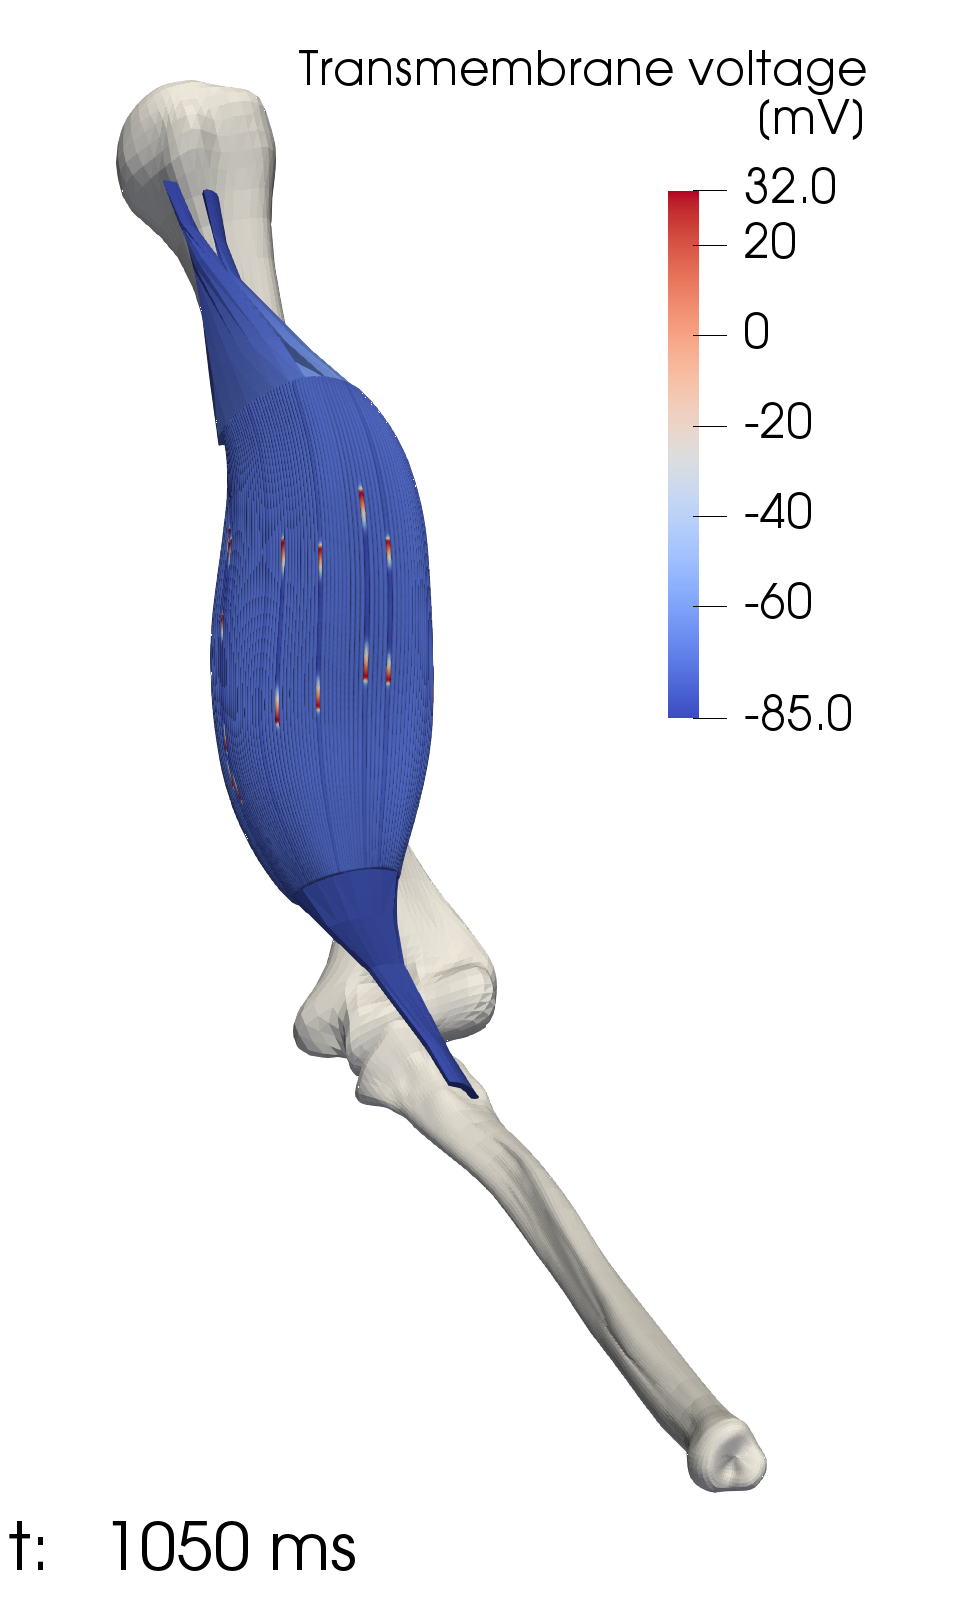
\includegraphics[height=97mm]{images/results/application/precice_activated_muscles1.png}%
    \caption{Muscle fibers colored by the value of the transmembrane potential $V_m$.}%
    \label{fig:precice_activated_muscles_1}%
  \end{subfigure}\,
  \begin{subfigure}[t]{0.28\textwidth}%
    \centering%
    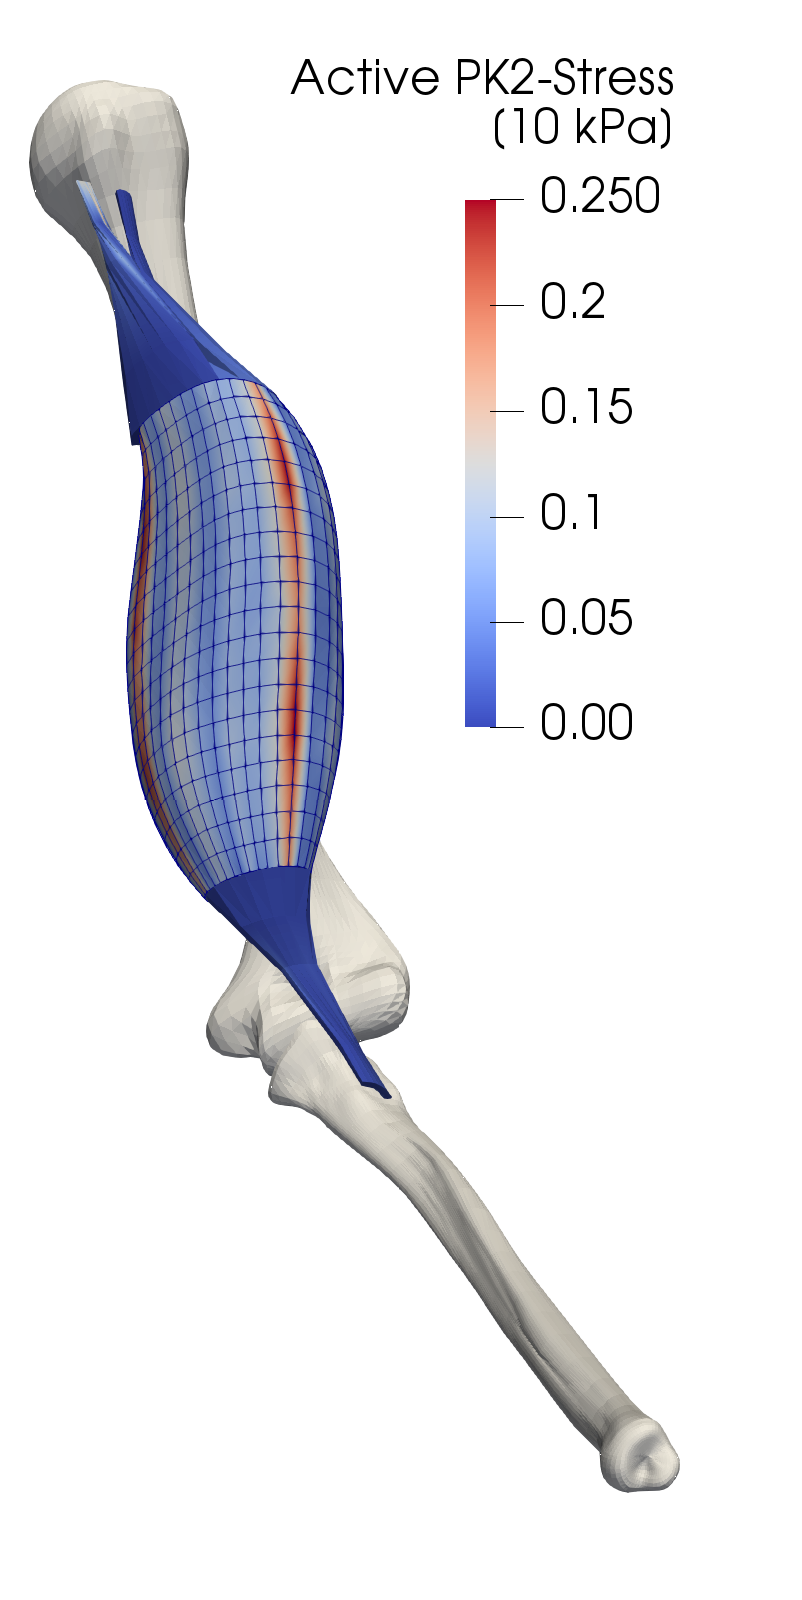
\includegraphics[height=97mm]{images/results/application/precice_activated_muscles2.png}%
    \caption{Active stress in the 3D muscle mesh.}%
    \label{fig:precice_activated_muscles_2}%
  \end{subfigure}
  \begin{subfigure}[t]{0.28\textwidth}%
    \centering%
    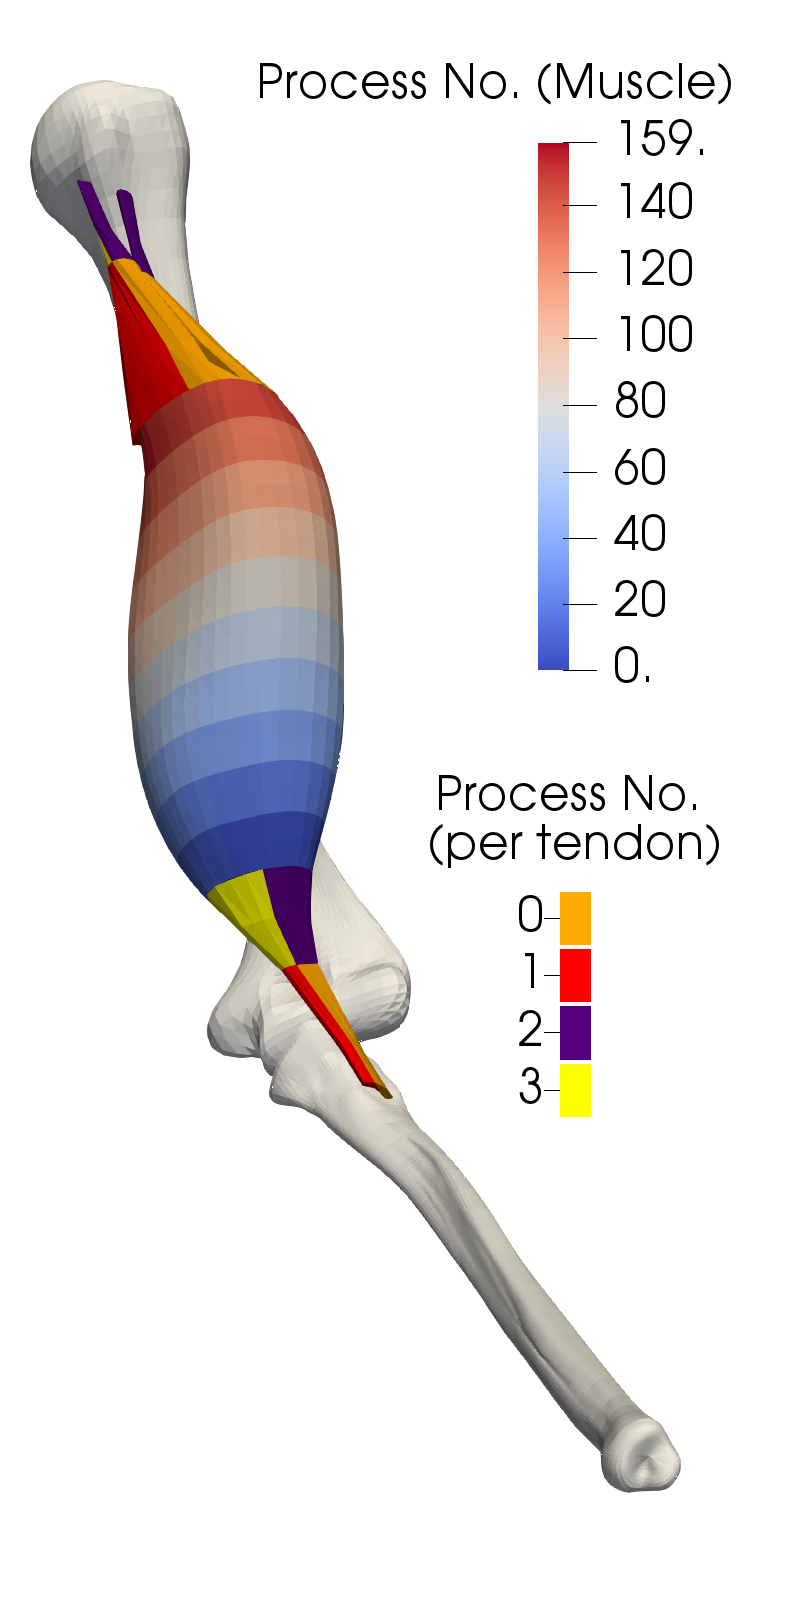
\includegraphics[height=97mm]{images/results/application/precice_activated_muscles3.png}%
    \caption{Parallel partitioning scheme.}%
    \label{fig:precice_activated_muscles_3}%
  \end{subfigure}
  \caption{Simulation of a muscle-tendon complex. Muscle and tendon geometries of the scenario with 1089 muscle fibers, embedded in the skeletal system comprising the ulna bone (lower end) and humerus bone (upper end), result of the simulation at $t=\SI{1.05}{\s}$.}%
  \label{fig:precice_muscle_force}%
\end{figure}%

The second scenario uses a coarser 3D mesh with 525 nodes and a parallel partitioning into eight subdomains. We simulate the resulting muscle force, measured at the top insertion point of the proximal tendons, over a longer time period of \SI{10}{\s}. \Cref{fig:precice_muscle_force0} shows the resulting relative force progression over time. The plot shows the total force as a moving average function over $\SI{0.1}{\s}$. It can be seen that the force initially increases, as more and more MUs get activated. A short delay between the onset of the last MU at $\SI{1.8}{\s}$ and the maximum force at \SI{2.39}{\s} can be seen. The muscle force exhibits large oscillations during the period of high muscle activation. They result from the lower firing frequencies of the later activated, large MUs and their higher contribution to the overall activity, compared to the smaller MUs. 

% muscle force
\begin{figure}
  \centering%
  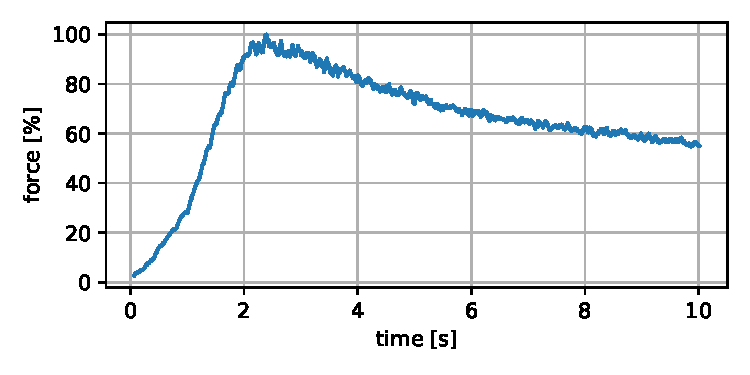
\includegraphics[width=0.7\textwidth]{images/results/application/precice_muscle_force.pdf}%
  \caption{Simulation of muscle force in a muscle-tendon complex. Resulting relative muscle force of the biceps muscle with attached tendons using the second scenario with 81 muscle fibers.}%
  \label{fig:precice_muscle_force0}%
\end{figure}

\Cref{fig:precice_muscle_force0} also shows that the generated muscle force rapidly decreases after the maximum is reached. This is a result from muscle fatigue, which is described by the Shorten subcellular model. The observed decrease to below \SI{60}{\percent} after \SI{10}{\s} can also be found in experimental studies of healthy subjects, e.g., in \cite{Enoka2008}. 

In conclusion, several biophysical simulation scenarios of MU activity induced muscle contraction have been presented in the previous sections. OpenDiHu allowed us to couple the computationally efficient fiber based electrophysiology description with the solid mechanics model of muscle deformation, as well as the biophysically more accurate multidomain model. An algorithm to include prestresses was presented and the coupling software preCICE was used to numerically couple individual parts of the multi-scale model. 

The last presented scenario simulated the generated force of a muscle-tendon complex for a simulation time span of \SI{10}{\s}. 
It can be used in the future to test hypotheses on the influence of various processes along the pathway from MU recruitment over muscle activation to force generation and macroscopic deformation. The simulated force progression related to the maximum voluntary contraction force is a macroscopic quantity, which can be easily measured in in vivo studies. Thus, a connection between the simulation domain and the experimental domain is given, and the microscopic subcellular processes in the muscle fibers are linked to a quantifiable outcome that can be compared with experiments.

\begin{reproduce_no_break}
  The simulations in this section were carried out on the supercomputer Hawk in Stuttgart. The job scripts can be found in the repository at \\ \href{https://github.com/dihu-stuttgart/performance}{github.com/dihu-stuttgart/performance} in the directory \code{opendihu/15_precice_biceps/with_electrophysiology}. To run similar simulations on other computers, run commands that are similar to the following (adjust the numbers of processes):
  \begin{lstlisting}[columns=fullflexible,breaklines=true,postbreak=\mbox{\textcolor{gray}{$\hookrightarrow$}\space}]
    cd $\$$OPENDIHU_HOME/examples/electrophysiology/fibers/fibers_contraction/with_tendons_precice/multiple_tendons_with_electrophysiology
    mpirun -n 1 muscle_electrophysiology_precice settings_muscle.py ramp.py
    mpirun -n 1 tendon_linear_precice_dynamic settings_tendon_bottom.py
    mpirun -n 1 tendon_linear_precice_dynamic settings_tendon_top_a.py
    mpirun -n 1 tendon_linear_precice_dynamic settings_tendon_top_b.py
  \end{lstlisting}
\end{reproduce_no_break}

